%Document's class%
\documentclass[conference]{IEEEtran}
\IEEEoverridecommandlockouts

%---------------------------------------------------------%

%Packages used%
\usepackage{cite}
\usepackage{amsmath,amssymb,amsfonts}
\usepackage{algorithmic}
\usepackage{graphicx}
\usepackage{textcomp}
\usepackage{xcolor}
\usepackage[table,xcdraw]{xcolor}
\usepackage{tikz}
\usetikzlibrary{positioning}
\usepackage{subcaption}
\usepackage{float}
\usepackage{caption}
\captionsetup[figure]{font=footnotesize}
\usepackage{multirow}
\usepackage{hyperref}
\usepackage{booktabs}
\usepackage{colortbl}
\usepackage[utf8]{inputenc}

%BibTeX logo function%
\def\BibTeX{{\rm B\kern-.05em{\sc i\kern-.025em b}\kern-.08em
    T\kern-.1667em\lower.7ex\hbox{E}\kern-.125emX}}

%---------------------------------------------------------%
%Codument start%
\begin{document}

%Main title%
\title{Comparing performance of 2 Deep Learning models to determine the impact of Transfer Learning when Identifying Human emotions}

%Authors list and Institutions legend%
\author{
 \IEEEauthorblockN{
  Sebastian 
  Russo \IEEEauthorrefmark{3}$^{,}$\IEEEauthorrefmark{1}
  $^{,}$\IEEEauthorrefmark{7},
  Javier
  Peres \IEEEauthorrefmark{3}$^{,}$\IEEEauthorrefmark{7},
  Guillermo 
  Trigo \IEEEauthorrefmark{3}$^{,}$\IEEEauthorrefmark{7},
  Raja Hashim 
  Ali\IEEEauthorrefmark{2}$^{,}$\IEEEauthorrefmark{4},
 }
 \\
 \IEEEauthorblockA{\IEEEauthorrefmark{3}
  University of Europe for Applied Sciences, Potsdam, Germany.
 }
 \IEEEauthorblockA{\IEEEauthorrefmark{2}
  Faculty of Computer Science \& Engineering, GIK Institute of Engg. Sciences \& Technology, Topi, Pakistan.
 }
 \IEEEauthorblockA{\IEEEauthorrefmark{4}
  Dept. of Technology \& Software Engineering, University of Europe for Applied Sciences, Berlin, Germany.
 }
 \IEEEauthorblockA{\IEEEauthorrefmark{1}
  Corresponding author: sebasruse03@gmail.com
 }
  \IEEEauthorblockA{\IEEEauthorrefmark{7}
  All authors contributed equally to this paper.
 }
}

\maketitle %Generate/print title and authors%

%Tikz environment to place the top most text%
\begin{tikzpicture}[overlay,remember picture]
    \path(current page.north) node(anchor){};
    \node[below=of anchor]{July, 2024 University of Europe for Applied Sciences (UE)};
\end{tikzpicture}

%---------------------------------------------------------%

%Abstract section%
\begin{abstract}
The Human emotion recognition from facial images constitutes an important task in computer vision and affective computing. This paper presents the implementation and comparative analysis of two similar deep learning models designed to identify human emotions from 48x48 gray-scale images of human faces. This study focuses on addressing the impact of transfer learning on the accuracy, loss and overall performance of emotion detection. Both models (built in Google Colab) implement a DenseNet169 classifier, a type of Convolutional Neural Network (CNN), and are also trained/tested on the same dataset of 35,685 data points of 48x48p gray-scale images categorized by emotion (happiness, neutral, sadness, anger, surprise, disgust, fear). The first model is trained from scratch and optimized for extracting spatial features from the images. The second model leverages transfer learning by initially freezing the weights of a pre-trained DenseNet169 network to subsequently unfreeze the weights and fine-tune it with a network for the specific task of emotion recognition. The performance of both models is evaluated in terms of accuracy, loss and overall performance, pointing the relative strengths and weaknesses of the approach of each model. Our findings highlight a significant advantage of transfer learning over not using it in achieving a higher accuracy in emotion detection, also we provide insights into potential applications and future directions for improving deep learning-based emotion recognition systems.
\end{abstract}

%Keyword index section%
\begin{IEEEkeywords}
Deep learning, Machine Learning, Emotion recognition, Transfer learning, DenseNet, DenseNet169, Convolutional Neural Network, CNN, Human emotions, Human, Emotions, Affective computing, Model Performance, 
\end{IEEEkeywords}

%---------------------------------------------------------%

%Intro of the paper%
\section{Introduction}
In recent years, the field of computer vision has witnessed significant advancements, particularly in tasks involving human-computer interaction and affective computing \cite{wang2022systematic}. One pivotal application within this domain is the recognition of human emotions from facial images, which holds profound implications for various sectors including healthcare, entertainment, and human-computer interaction systems, such as Virtual reality to just mention one of them \cite{marin2020emotion}.

The ability to accurately interpret and respond to human emotions plays a crucial role in enhancing user experience and interaction with technological systems. Emotion recognition from facial expressions not only enables personalized services and content delivery but also facilitates psychological analysis and clinical diagnostics, allowing computer systems to recognize the emotion a human is portraying and most likely feeling and respond accordingly \cite{nandwani2021review}.

A Deep learning model, and specifically Convolutional Neural Networks (CNNs), have emerged as one of the most powerful tools for automated facial emotion recognition tasks. These networks can effectively learn hierarchical representations from raw image data, enabling them to discern subtle patterns and features indicative of different emotional states. Among the available CNN architectures, our investigation proves that DenseNet169 shows great promise due to its densely connected layers that facilitate feature reuse and gradient propagation, thereby enhancing model performance the most \cite{li2021efficient}.

Despite the effectiveness of CNNs, the task of training deep learning models for emotion recognition often faces challenges related to data scarcity, class imbalance, and overfitting. Therefor, Transfer learning, a technique that leverages pre-trained models on large-scale datasets, has emerged as a potential solution to mitigate these challenges. By transferring knowledge learned from one task (e.g., ImageNet classification) to another (e.g., emotion recognition), transfer learning can expedite model convergence, improve generalization, and enhance overall performance \cite{neyshabur2020being}.

This paper presents a comparative analysis of two Deep Learning models based on the DenseNet169 architecture, evaluating their performance in identifying human emotions from 48x48 grayscale facial images. The study specifically investigates the impact of transfer learning on model accuracy, loss, and overall performance metrics. One model is trained from scratch, while the other utilizes transfer learning by fine-tuning a pre-trained DenseNet169 model initially trained on ImageNet, but both share most of their architecture except for the usage of transfer learning. The comparative evaluation is conducted using a dataset of 35,685 images categorized into seven emotion classes: happiness, neutral, sadness, anger, surprise, disgust, and fear.

By systematically comparing these models, this study aims to provide insights into the efficacy of transfer learning for emotion recognition tasks and to delineate best practices for deploying deep learning models in affective computing applications. The findings contribute to advancing the field of automated emotion recognition, highlighting the potential of transfer learning to enhance model robustness and applicability in real-world scenarios.


%-------%


%Problem statement%
\section{Problem Statement}
The ability to recognize Human emotions from facial images is extremely relevant for computer vision and affective computing, very pivotal for applications based on human-computer interactions and even useful for psychological analysis. This study seeks to compare the performance of two deep learning models built in Python (Google Colab), implementing DenseNet169 in both cases (a Convolutional Neural Network), to identify human emotions specifically from 48x48 gray-scale facial images. Sowmiya et al. demonstrated DenseNet169 as an effective model for this task \cite{sowmiya2022facial}. Our primary objective is to evaluate the extend of the impact transfer learning has on the emotion detection accuracy. One model is trained from scratch to extract spatial features directly from images, while the other employs transfer learning by leveraging a pre-trained DenseNet169 network. Initially freezing its weights, the network is afterwards fine-tuned for emotion recognition. The systematic comparison of these approaches are based on a single dataset of 35,685 images categorized into emotional states (happiness, neutral, sadness, anger, surprise, disgust, fear). This research aims to assess the efficacy of transfer learning in enhancing emotion recognition accuracy and to delineate best practices for deploying deep learning models in affective computing applications.


%-------%

%Our Contributions%
\section{Our Contributions}
In this study, we present a comprehensive analysis of emotion recognition from facial images, employing the DenseNet169 architecture with transfer learning. Our contributions are multifaceted and address various aspects of this challenging task. The key contributions of our work are as follows:

\begin{enumerate}
    \item \textbf{Implementation of Transfer Learning for Emotion Recognition:} We employed the DenseNet169 model pre-trained on the ImageNet dataset and fine-tuned it for the task of emotion recognition using grayscale facial images. This approach leverages the rich feature representations learned from a large and diverse dataset, enhancing the model's performance on a more specific and smaller emotion recognition dataset.

    \item \textbf{Comparative Analysis with Non-Transfer Learning Approach:} We conducted a thorough direct comparison between the performance of the transfer learning model and a model trained from scratch. Our analysis demonstrated that the transfer learning model significantly outperforms the non-transfer learning model across various metrics, including accuracy, loss, confusion matrix, ROC curves, and precision-recall curves.

    \item \textbf{Detailed Performance Metrics and Visualization:} We provided an in-depth evaluation of the models using multiple metrics to offer a comprehensive understanding of their performance. This includes accuracy, loss, confusion matrix analysis, ROC curves, and precision-recall curves, each offering unique insights into the model's strengths and areas for improvement.

    \item \textbf{Addressing Class Imbalance:} We identified and discussed the challenge of class imbalance in emotion recognition datasets, particularly with the disgust emotion. Our study highlights the impact of this imbalance on model performance and suggests potential techniques for mitigating this issue in future research and studies.

    \item \textbf{Insights for Practical Applications:} Our findings have practical implications for various fields, including affective computing, human-computer interaction, healthcare, entertainment, and security. We discussed how improved emotion recognition systems can enhance user experience, aid in mental health monitoring, create more immersive virtual environments, and improve threat detection systems.

    \item \textbf{Recommendations for Future Research:} We provided several recommendations for future research directions. These include exploring diverse datasets to enhance generalization, investigating alternative deep learning architectures and ensemble learning approaches, and optimizing models for deployment on different hardware platforms.

\end{enumerate}

In summary, our study demonstrates the effectiveness of transfer learning in improving emotion recognition from facial images. By leveraging pre-trained models and conducting a detailed comparative analysis, we provide valuable insights and contributions to the field of automated emotion recognition, paving the way for future advancements and practical implementations.


%-------%

%Methodology Section%
\section{Methodology}
This section outlines the methodology employed in this study, detailing the dataset, pre-processing steps, model architecture, training procedure, and evaluation metrics used to assess the performance of the DenseNet169 model with and without transfer learning.

%Dataset explanation%
\subsection{Dataset}
The dataset used for this study is the \href{https://www.kaggle.com/datasets/ananthu017/emotion-detection-fer}{motion-detection-fer} dataset, which comprises a diverse collection of facial images annotated with corresponding emotion labels. The dataset includes 35,685 examples of 48x48 pixel gray-scale images of faces divided into training and testing datasets. Images are categorized based on the emotion shown in the facial expressions into seven classes: happiness, neutral, sadness, anger, surprise, disgust, and fear. The distribution of data \ref{fig:datasetdistr} of the dataset presents information that probably allow us to predict the results of both models.
\begin{figure}[H]
    \centering
    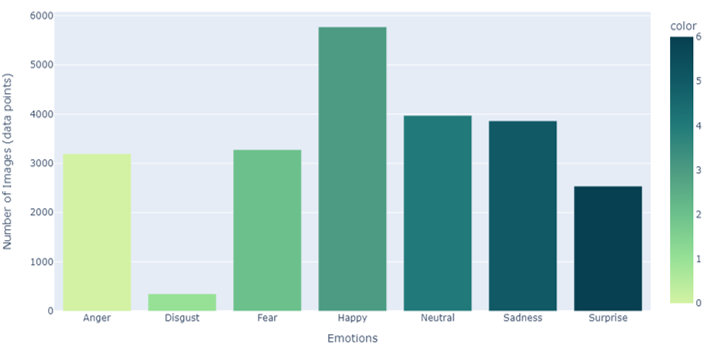
\includegraphics[width=0.45\textwidth]{Figures/Dataset distribution.png}
    \caption{Dataset distribution of data points among 7 classes of emotions (Anger, Disgust, Fear, Happy, Neutral, Sadness and Surprise)}
    \label{fig:datasetdistr}
\end{figure}

%Preprocessing of data%
\subsection{Data Pre-processing}
Pre-processing is a crucial step to ensure the quality and consistency of the input data. The following pre-processing steps were applied on both models in the same way:

\begin{itemize}
    \item \textbf{Resizing}: All images were resized to 48x48 pixels to maintain consistency with the dataset specifications.
    \item \textbf{Normalization}: Pixel values were normalized to the range [0, 1] by dividing them by 255 parts.
    \item \textbf{Augmentation}: To enhance the robustness of the model, data augmentation techniques such as rotation, flipping, and zooming were applied during training.
\end{itemize}

%Model architecture%
\subsection{Architectures}
The DenseNet169 architecture, known for its densely connected convolutional networks, was utilized in this study. The architecture consists of 8 layers total distinct layers, counting each Dense and Dropout, with 5 main functionally important layers that feature skip connections that improve gradient flow and reduce the vanishing gradient problem.
\begin{itemize}
    \item \textbf{GlobalAveragePooling2D}: The Layer executes a global average pooling on the spatial dimensions of the input tensor of all values in each feature map and outputs.
    \item \textbf{DenseLayer-256 Neurons}: Fully connected layer with 256 neurons, activation function ReLu for non-linearity and L2 regularization (weight decay) to prevent over-fitting.
    \item \textbf{Dropout Layer-30\%}: Randomly drops 30\% of the neurons during training to prevent over-fitting.
    \item \textbf{DenseLayer-1024 Neurons}: Fully connected layer with 1024 neurons and the same activation and regularization as the first DenseLayer.
    \item \textbf{Dropout Layer-50\%}: Randomly drops 50\% of the neurons during training to prevent over-fitting.
    \item \textbf{DenseLayer-512 Neurons}: Fully connected layer with 512 neurons and the same activation and regularization as the first DenseLayer.
    \item \textbf{Dropout Layer-50\%}: Randomly drops 50\% of the neurons during training to prevent over-fitting.
    \item \textbf{Output DenseLayer-7 neurons}: Output layer that features 7 neurons for the 7 classes (One vs all), using activation function Softmax.
\end{itemize}

%Transfer learning specific%
\subsubsection{Transfer Learning Setup (Freeze-UnFreeze)}
For the transfer learning model, weights pre-trained on the ImageNet dataset were used. The following modifications were made to adapt the pre-trained model for emotion classification:

\begin{itemize}
    \item \textbf{Input Layer}: The input layer was modified to accept 48x48 pixel grayscale images.
    \item \textbf{Freezing Layers}: The initial usage of the model and its layers of DenseNet169 model were frozen to retain the learned features from the ImageNet dataset.
    \item \textbf{Custom Classification Head}: The final classification layer was replaced with a new dense layer having seven neurons, corresponding to the number of emotion categories in our dataset and therefore implementing the "One vs All" technique.
\end{itemize}

%Non-transfer learning specific%
\subsubsection{Non-Transfer Learning Setup (from scratch)}
For the model trained from scratch, the DenseNet169 architecture was initialized with random weights. The entire model was trained end-to-end on the emotion recognition dataset without leveraging any pre-trained weights.


%Training procedure%
\subsection{Training Procedure}
The models were trained using the following settings:

\begin{itemize}
    \item \textbf{Optimizer}: The SGD (Stochastic Gradient Descent) optimizer was used for training, with an initial learning rate of 0.001 for the model that doesn't implement Transfer Learning. In the case of the model that implements Transfer learning, the learning rate was initially 0.01 for the freezed layers and then lowered to 0.001 for the unfreezed layer.
    \item \textbf{Loss Function}: Categorical cross-entropy loss was employed to measure the error between predicted and true labels in both models.
    \item \textbf{Batch Size}: A batch size of 64 was used for both models.
    \item \textbf{Epochs}: The model that doesn't implement Transfer Learning was trained for 20 epochs; Meanwhile, the model that implements Transfer Learning can be trained in a range between 23 epochs at minimum to 50 epochs at maximum. This is because the pre-train portion (freezed layers) has 30 epochs to go through, however, it also has an early stop function that stops the training if there is no improvement after 3 epochs and restores the model's weight of the best epoch in this training, afterwards the model is trained for 20 more epochs like the other model.
\end{itemize}

Early stopping was implemented to prevent over-fitting, with a patience of 3 epochs based on validation loss.


%Evaluation metrics and graphs%
\subsection{Evaluation Metrics}
The performance of the models was evaluated using the following metrics:

\begin{itemize}
    \item \textbf{Accuracy vs number of epochs}: The overall accuracy of the model in correctly classifying the emotions.
    \item \textbf{Loss vs number of epochs}: The categorical cross-entropy loss on the validation set.
    \item \textbf{Confusion Matrix}: A confusion matrix was used to visualize the performance across different emotion classes.
    \item \textbf{ROC curve}: the Receiver Operating Characteristic curve, represents graphically used to evaluate the performance of the classification model, plotting the true positive rate (TPR) against the false positive rate (FPR).
    \item \textbf{Precision-Recall Curve}: Precision-recall curves were plotted to evaluate the trade-off between precision and recall for each class.
\end{itemize}


%Hardware specific details%
\subsection{Implementation Details}
The models were implemented using the TensorFlow and Keras libraries. Training, and the whole code, was conducted on Google Colab, utilizing the CPU and T4 GPU runtime type. 

All experiments were conducted in a controlled environment to ensure reproducibility and consistency of the results.


%Summary%
\subsection{Summary}
The methodology outlined above provides a comprehensive framework for evaluating the effectiveness of transfer learning in emotion recognition tasks. By comparing the performance of models with and without transfer learning, we aim to demonstrate the benefits of leveraging pre-trained models in deep learning applications. The workflow of both Deep learning models are as follows:
\begin{figure}[H]
    \centering
    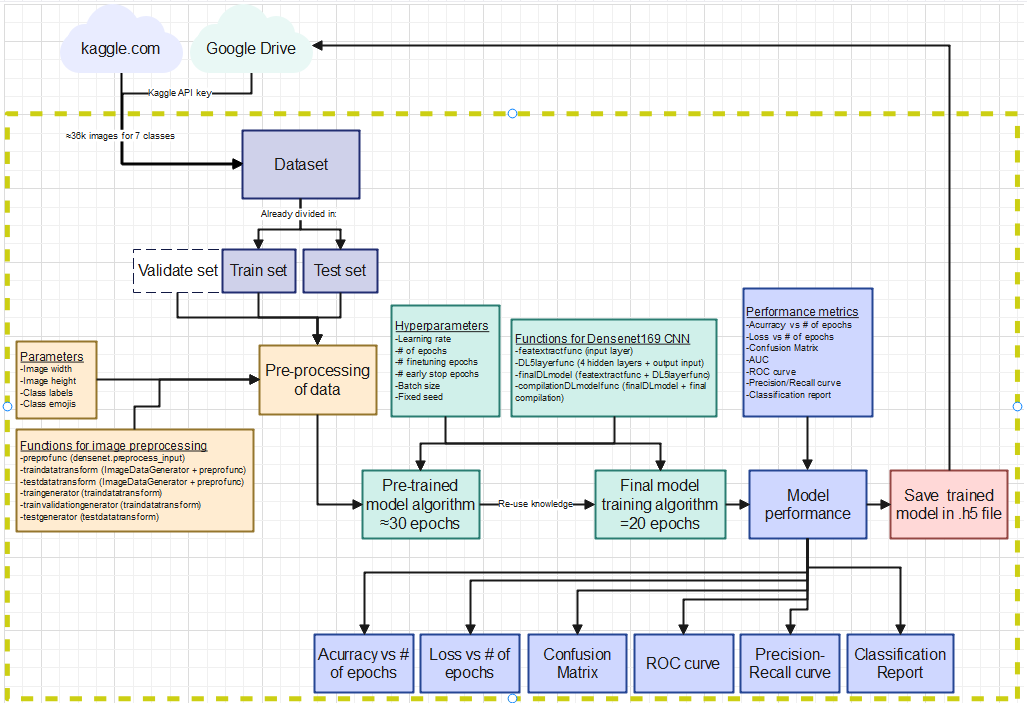
\includegraphics[width=0.45\textwidth]{Figures/Trans_learn_workflow.png}
    \caption{Workflow for the Deep learning model with Transfer Learning}
    \label{fig:workflow_DLTL}
\end{figure}
\begin{figure}[H]
    \centering
    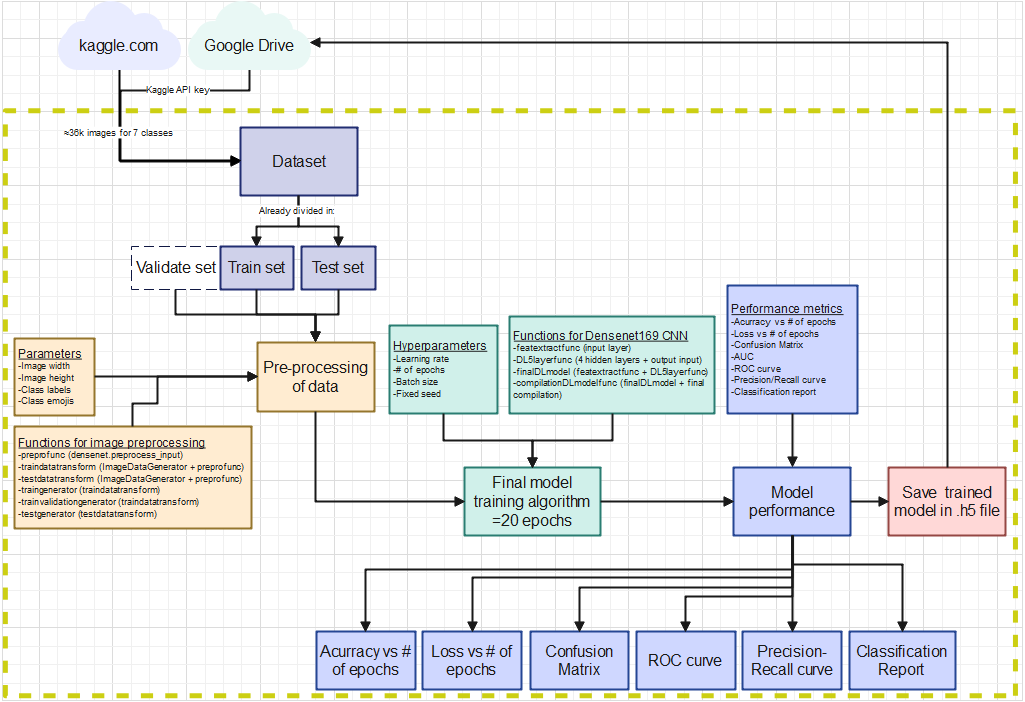
\includegraphics[width=0.45\textwidth]{Figures/no_Trans_learn_workflow.png}
    \caption{Workflow for the Deep learning model without Transfer Learning}
    \label{fig:workflow_DLnoTL}
\end{figure}


%-------%

%Results Section
\section{Results}
The primary objective of this study was to evaluate the impact of transfer learning on the performance of a DenseNet169 model in identifying human emotions from facial images. The performance metrics include accuracy, loss, confusion matrix, ROC and precision-recall curves, all of which are compared for models with and without transfer learning.

\subsection{Model Performance with Transfer Learning}

% Subsection: Model Performance with Transfer Learning

\subsubsection{Accuracy and Loss}
The model incorporating transfer learning demonstrated significantly higher accuracy and lower loss over the training epochs compared to the model trained from scratch. Figures \ref{fig:accuracy_tl} and \ref{fig:loss_tl} illustrate the accuracy and loss progression respectively.

\begin{figure}[H]
    \centering
    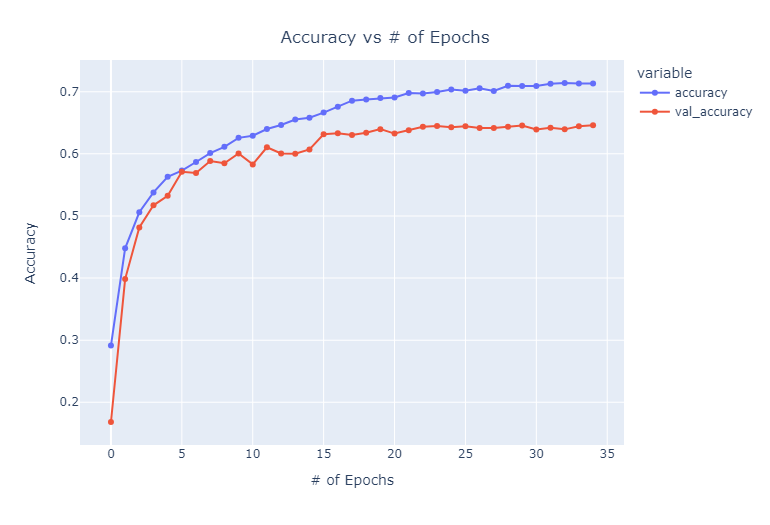
\includegraphics[width=0.45\textwidth]{Figures/accuracyvsnumepochs.png}
    \caption{Accuracy vs. Number of Epochs for Model with Transfer Learning}
    \label{fig:accuracy_tl}
\end{figure}

\begin{figure}[H]
    \centering
    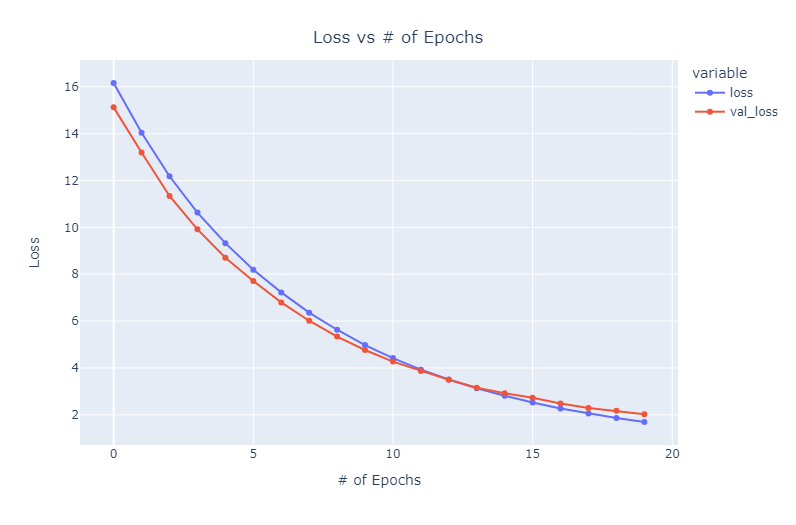
\includegraphics[width=0.45\textwidth]{Figures/loss vs numepochs.png}
    \caption{Loss vs. Number of Epochs for Model with Transfer Learning}
    \label{fig:loss_tl}
\end{figure}

\subsubsection{Confusion Matrix}
The confusion matrix for the transfer learning model (Figure \ref{fig:confmat_tl}) shows a higher number of correct classifications across all emotion categories, indicating improved performance.

\begin{figure}[H]
    \centering
    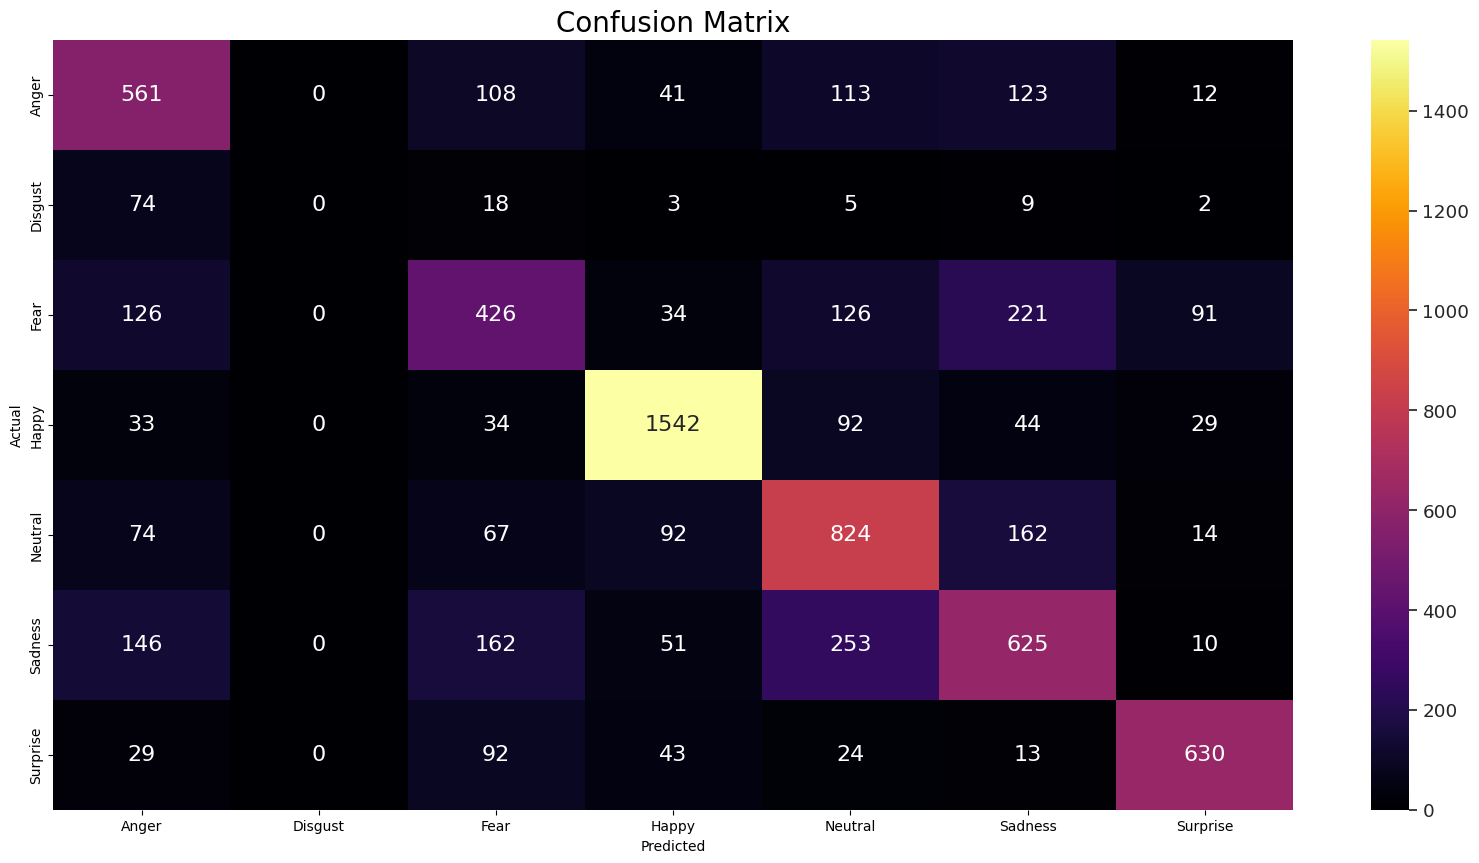
\includegraphics[width=0.45\textwidth]{Figures/Confusion Matrix.png}
    \caption{Confusion Matrix for Model with Transfer Learning}
    \label{fig:confmat_tl}
\end{figure}

\subsubsection{ROC (Receiver Operating Characteristic)}
The Receiver Operating Characteristic curve (Figure \ref{fig:roc_tl} shows the model with transfer learning has a higher true positive rate (TPR) against the false positive rate (FPR) the model might have incurred to.

\begin{figure}[H]
    \centering
    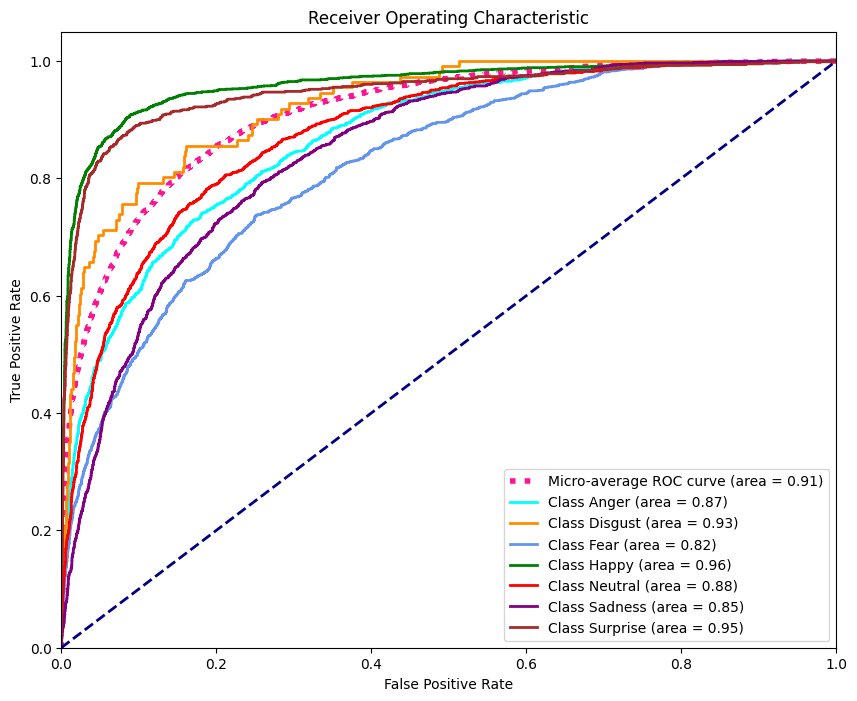
\includegraphics[width=0.45\textwidth]{Figures/ROC.png}
    \caption{ROC Curve for Model with Transfer Learning}
    \label{fig:roc_tl}
\end{figure}
\subsubsection{Precision-Recall Curve}
The precision-recall curve (Figure \ref{fig:prec_recall_tl}) further supports the effectiveness of transfer learning, showing a better balance between precision and recall across all classes.

\begin{figure}[H]
    \centering
    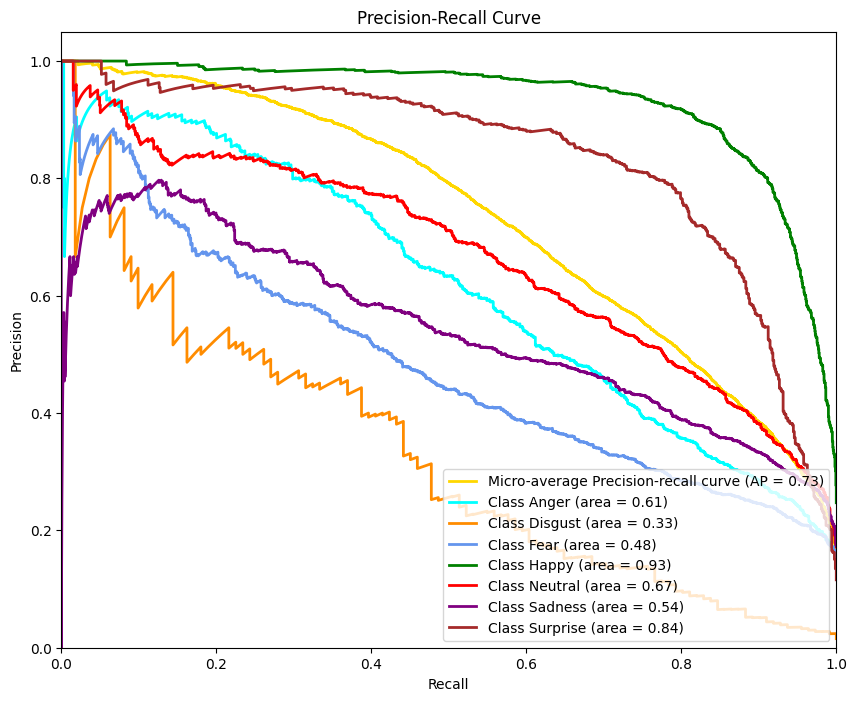
\includegraphics[width=0.45\textwidth]{Figures/Precision-recall curve.png}
    \caption{Precision-Recall Curve for Model with Transfer Learning}
    \label{fig:prec_recall_tl}
\end{figure}

\subsection{Model Performance without Transfer Learning}

% Subsection: Model Performance without Transfer Learning

\subsubsection{Accuracy and Loss}
For comparison, the model trained without transfer learning exhibited lower accuracy and higher loss, as depicted in Figures \ref{fig:accuracy_no_tl} and \ref{fig:loss_no_tl}.

\begin{figure}[H]
    \centering
    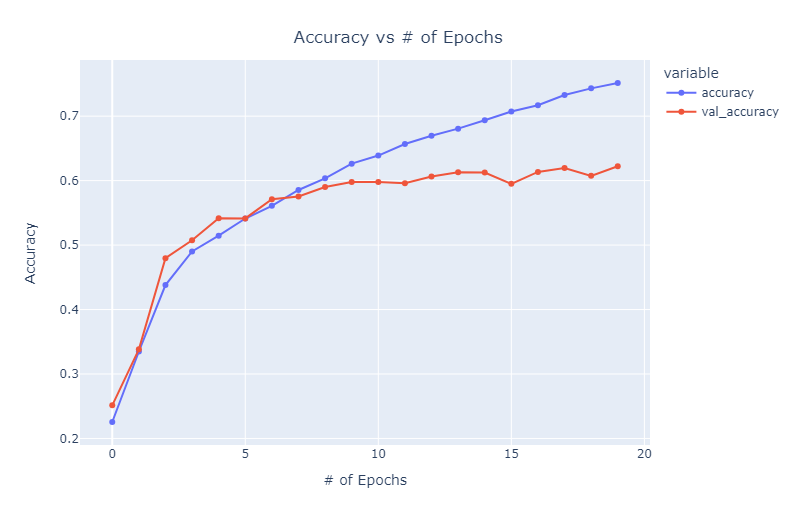
\includegraphics[width=0.45\textwidth]{Figures/acurracy vs numepochs - no TL.png}
    \caption{Accuracy vs. Number of Epochs for Model without Transfer Learning}
    \label{fig:accuracy_no_tl}
\end{figure}

\begin{figure}[H]
    \centering
    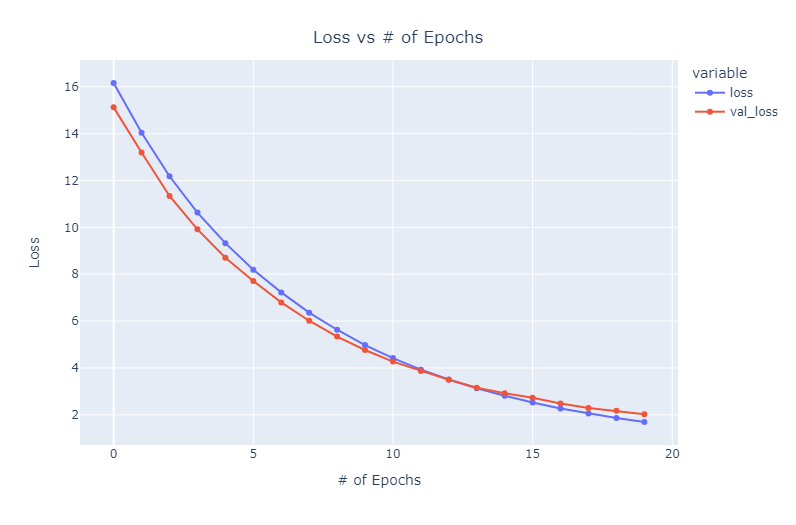
\includegraphics[width=0.45\textwidth]{Figures/loss vs numepochs - no TL.png}
    \caption{Loss vs. Number of Epochs for Model without Transfer Learning}
    \label{fig:loss_no_tl}
\end{figure}

\subsubsection{Confusion Matrix}
The confusion matrix for the model without transfer learning (Figure \ref{fig:confmat_no_tl}) shows more erroneous classifications compared to the transfer learning model.

\begin{figure}[H]
    \centering
    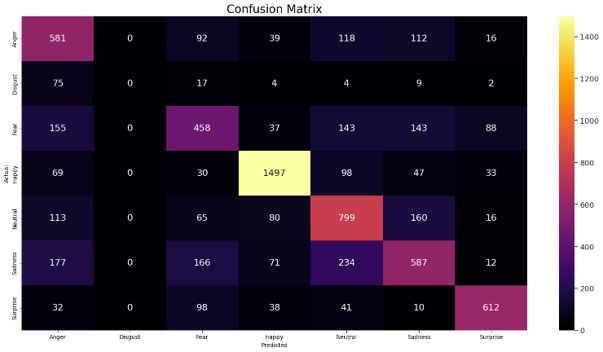
\includegraphics[width=0.45\textwidth]{Figures/Confusion matrix - no TL.png}
    \caption{Confusion Matrix for Model without Transfer Learning}
    \label{fig:confmat_no_tl}
\end{figure}

\subsubsection{ROC (Receiver Operating Characteristic)}
The Receiver Operating Characteristic curve (Figure \ref{fig:roc_notl} shows the model without transfer learning has noticeable lower true positive rate (TPR) against the false positive rate (FPR) when comparing it to the model that does implement Transfer Learning.

\begin{figure}[H]
    \centering
    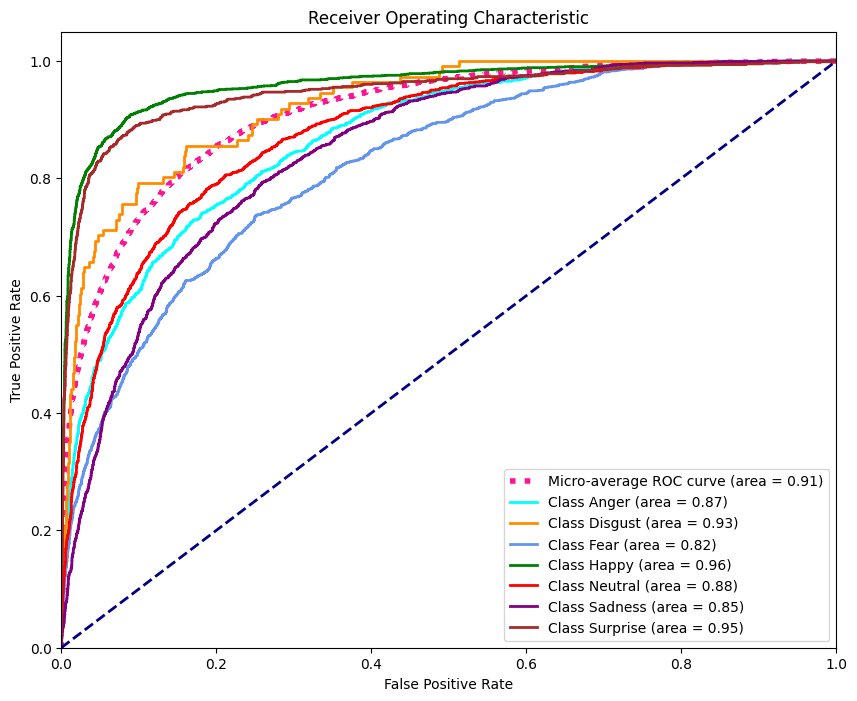
\includegraphics[width=0.45\textwidth]{Figures/ROC - no TL.png}
    \caption{ROC Curve for Model with Transfer Learning}
    \label{fig:roc_notl}
\end{figure}
\subsubsection{Precision-Recall Curve}
Similarly, the precision-recall curve (Figure \ref{fig:prec_recall_no_tl}) indicates poorer performance in balancing precision and recall for the model without transfer learning.

\begin{figure}[H]
    \centering
    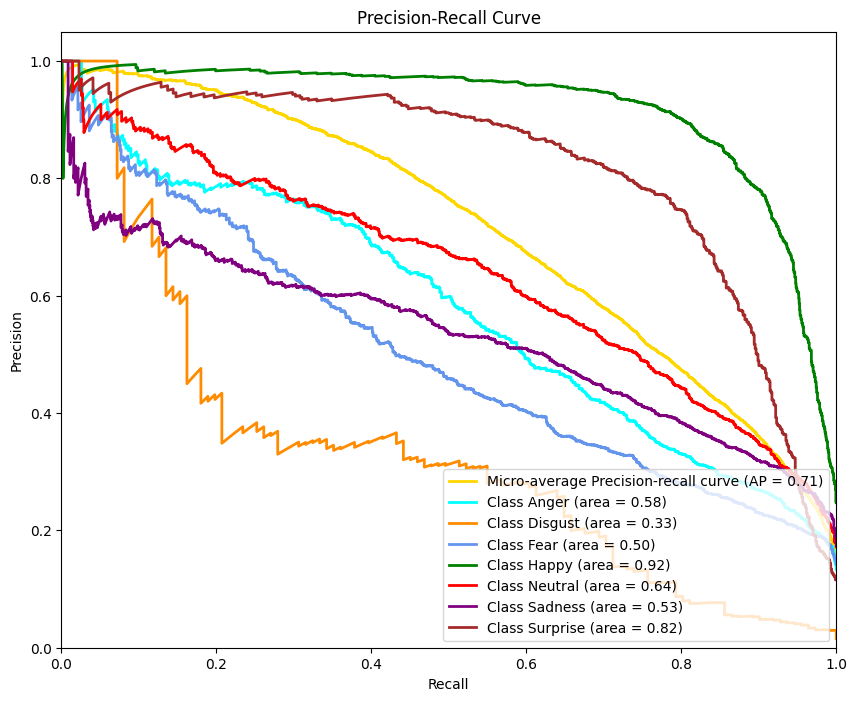
\includegraphics[width=0.45\textwidth]{Figures/Precision-recall curve - no TL.png}
    \caption{Precision-Recall Curve for Model without Transfer Learning}
    \label{fig:prec_recall_no_tl}
\end{figure}

\subsection{Predictions}

% Subsection: Predictions

\subsubsection{Predictions on Specific Images and Videos}
The model's predictions on selected images and videos provide insights into its performance in different scenarios for both models:

\begin{itemize}
    \item \textbf{Prediction of 9 Images:} Figures \ref{fig:9imageprediction_TLmodel} and \ref{fig:9imageprediction_NOTLmode} showcases each model's prediction capabilities on a variety of facial expressions, displaying key differences between both models:
    
    \begin{figure}[H]
        \centering
        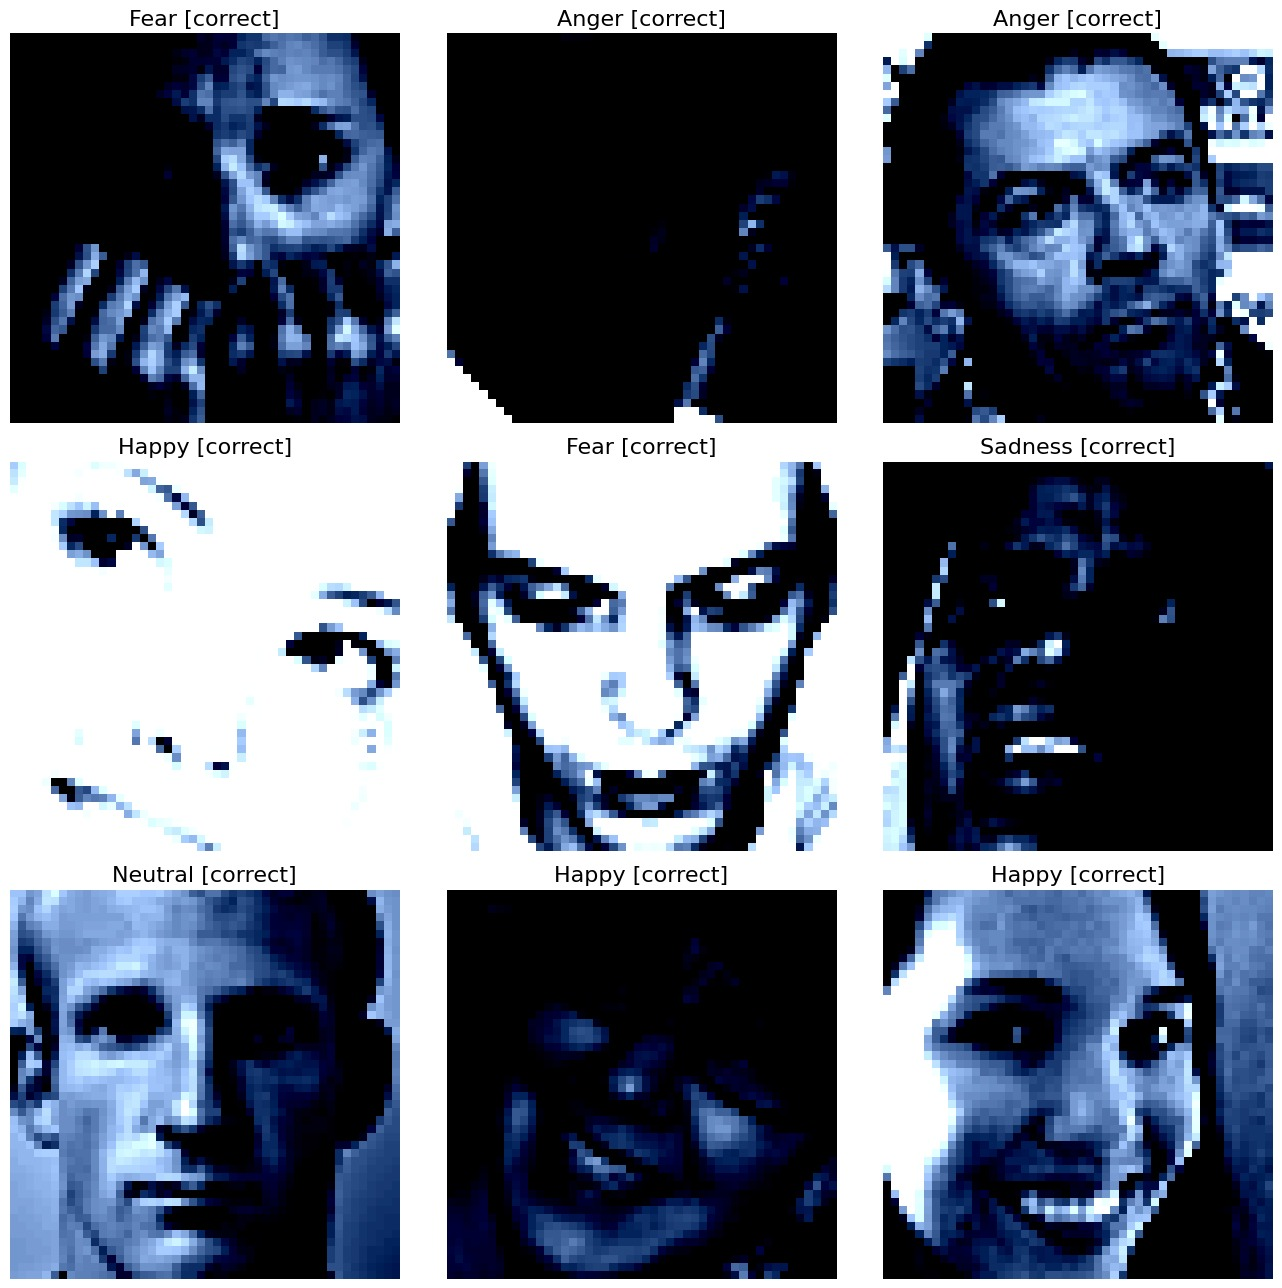
\includegraphics[width=0.4\textwidth]{Figures/9imagepredictionTLmodel.png}
        \caption{Prediction of 9 Images with Transfer Learning}
        \label{fig:9imageprediction_TLmodel}
    \end{figure}

    \begin{figure}[H]
        \centering
        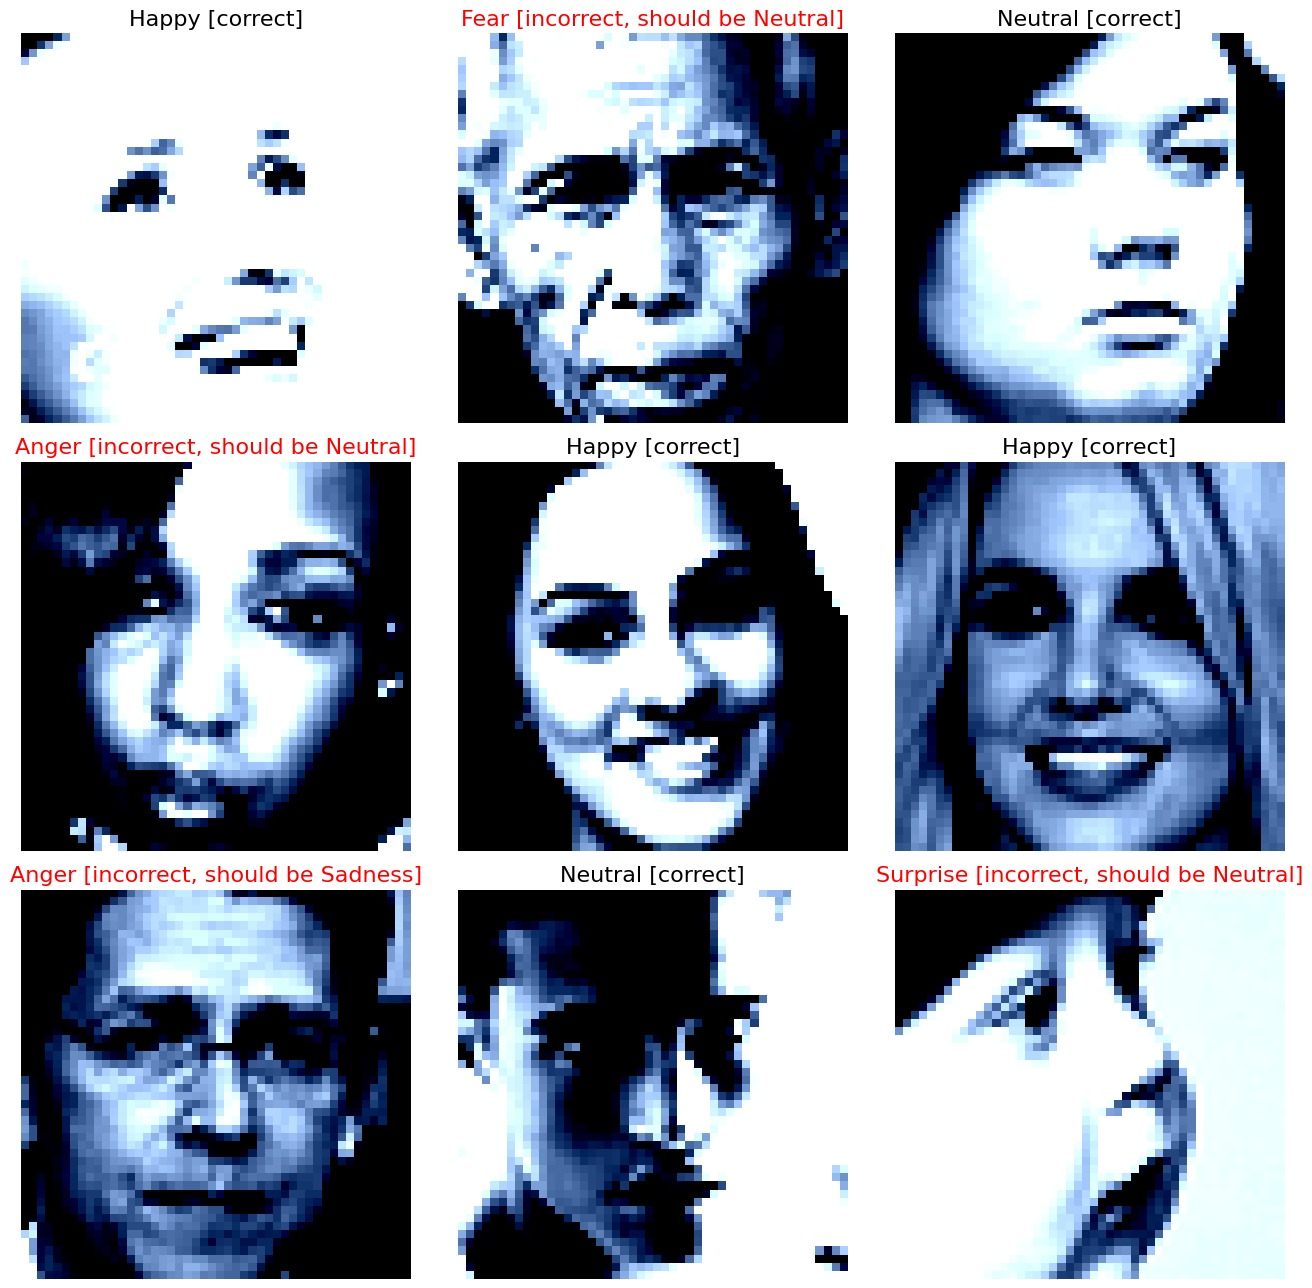
\includegraphics[width=0.4\textwidth]{Figures/9imagepredictionNOTLmodel.png}
        \caption{Prediction of 9 Images without Transfer Learning}
        \label{fig:9imageprediction_NOTLmode}
    \end{figure}
    
    \item \textbf{Real-Time Video Analysis:} An analysis of real-time video captured using OpenCV reveals varying performance across different emotion labels. Emotions such as neutral, happy, surprise (Figure \ref{fig:opencvsurprise}), anger, neutral and happy demonstrated more consistent and accurate predictions compared to others, as observed in the image file \ref{fig:prediction_8_images}.
    
    \begin{figure}[H]
        \centering
        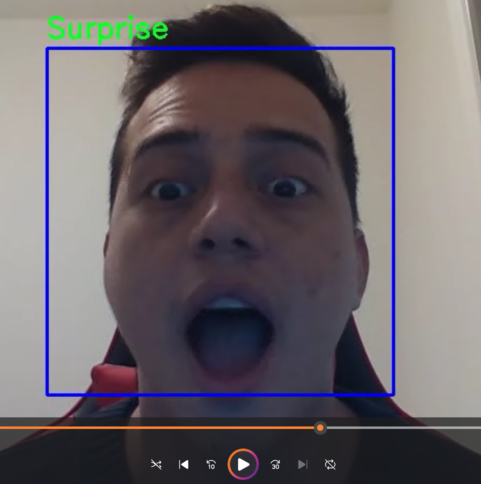
\includegraphics[width=0.4\textwidth]{Figures/opencvsurprise.png}
        \caption{Prediction in Real-Time Analysis (Surprise)}
        \label{fig:opencvsurprise}
    \end{figure}
    
    \item \textbf{3 Images Prediction:} Figure \ref{fig:3camimageprediction} shows the model correctly identifying the emotion as "happy" in 1 out of the 3 images, the other two got were incorrectly predicted.
    
    \begin{figure}[H]
        \centering
        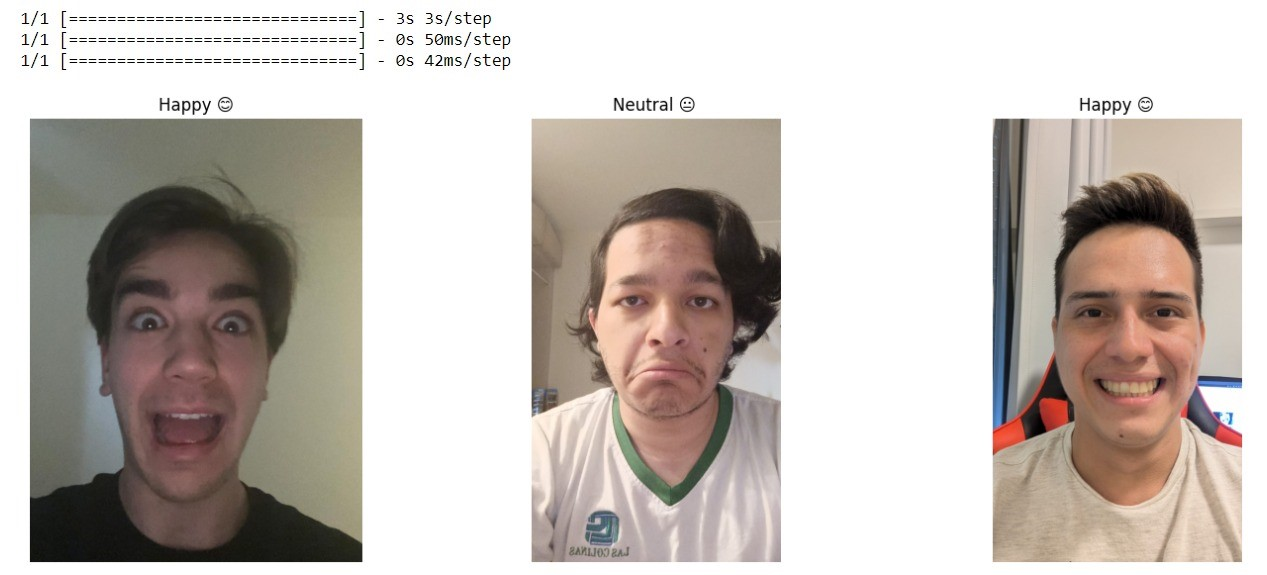
\includegraphics[width=0.5\textwidth]{Figures/3camimageprediction.png}
        \caption{3 cam Images Prediction}
        \label{fig:3camimageprediction}
    \end{figure}
    
\end{itemize}

\subsection{Summary of Results}

% Subsection: Summary of Results

The comparative analysis clearly demonstrates that transfer learning significantly enhances the performance of the DenseNet169 model for emotion recognition tasks. The model trained with transfer learning not only achieved higher accuracy and lower loss but also exhibited superior classification capabilities as evidenced by the confusion matrix and precision-recall curves. These findings underscore the importance of leveraging pre-trained models in deep learning applications, particularly in fields like affective computing where data scarcity and class imbalances are common challenges. As shown in the following comparative table:

%1st table%
\begin{table}[H]
\begin{tabular}{|
>{\columncolor[HTML]{FFFC9E}}c ll|}
\hline
\multicolumn{3}{|c|}{\cellcolor[HTML]{FFCCC9}Acurracy and Loss with validation}                                                                                                                                \\ \hline
\multicolumn{1}{|c|}{\cellcolor[HTML]{FFCCC9}Metrics/Models} & \multicolumn{1}{c|}{\cellcolor[HTML]{FFCE93}\begin{tabular}[c]{@{}c@{}}Transfer Learning\\ model\end{tabular}} & \multicolumn{1}{c|}{\cellcolor[HTML]{FFCE93}\begin{tabular}[c]{@{}c@{}}Non-Transfer Learning \\ model\end{tabular}} \\ \hline
\multicolumn{1}{|c|}{\cellcolor[HTML]{FFFC9E}Acurracy}       & \multicolumn{1}{l|}{Aprox. 0.72}                                     & Aprox. 0.74                                                              \\ \hline
\multicolumn{1}{|c|}{\cellcolor[HTML]{FFFC9E}Val-Acurracy}   & \multicolumn{1}{l|}{Aprox. 0.65}                                     & Aprox. 0.98                                                              \\ \hline
\multicolumn{1}{|c|}{\cellcolor[HTML]{FFFC9E}Loss}           & \multicolumn{1}{l|}{Aprox. 1.02}                                     & Aprox. 0.98                                                              \\ \hline
\multicolumn{1}{|c|}{\cellcolor[HTML]{FFFC9E}Val-Loss}       & \multicolumn{1}{l|}{Aprox. 0.98}                                     & Aprox. 0.98                                                              \\ \hline
\end{tabular}
\caption{Direct comparison between Acurracy, Loss, Valid Acurracy and Valid Loss between both models}
\label{tab:acurracy-vs-loss-models}
\end{table}

%2nd table%
\begin{table}[H]
\begin{tabular}{|
>{\columncolor[HTML]{FFFC9E}}c ll|}
\hline
\multicolumn{3}{|c|}{\cellcolor[HTML]{FFCCC9}True positives comparison from the Confusion Matrices}                                                                                                                \\ \hline
\multicolumn{1}{|c|}{\cellcolor[HTML]{FFCCC9}TP/Models}         & \multicolumn{1}{c|}{\cellcolor[HTML]{FFCE93}\begin{tabular}[c]{@{}c@{}}Transfer Learning\\ model\end{tabular}} & \multicolumn{1}{c|}{\cellcolor[HTML]{FFCE93}\begin{tabular}[c]{@{}c@{}}Non-Transfer Learning \\ model\end{tabular}} \\ \hline
\multicolumn{1}{|c|}{\cellcolor[HTML]{FFFC9E}Anger class TPs}    & \multicolumn{1}{l|}{561}                                             & 581                                                                      \\ \hline
\multicolumn{1}{|c|}{\cellcolor[HTML]{FFFC9E}Disgust class TPs}  & \multicolumn{1}{l|}{0}                                               & 0                                                                        \\ \hline
\multicolumn{1}{|c|}{\cellcolor[HTML]{FFFC9E}Fear class TPs}     & \multicolumn{1}{l|}{426}                                             & 458                                                                      \\ \hline
\multicolumn{1}{|c|}{\cellcolor[HTML]{FFFC9E}Happy class TPs}    & \multicolumn{1}{l|}{1542}                                            & 1497                                                                     \\ \hline
\multicolumn{1}{|c|}{\cellcolor[HTML]{FFFC9E}Neutral class TPs}  & \multicolumn{1}{l|}{824}                                             & 799                                                                      \\ \hline
\multicolumn{1}{|c|}{\cellcolor[HTML]{FFFC9E}Sadness class TPs}  & \multicolumn{1}{l|}{625}                                             & 587                                                                      \\ \hline
\multicolumn{1}{|c|}{\cellcolor[HTML]{FFFC9E}Surprise class TPs} & \multicolumn{1}{l|}{630}                                             & 612                                                                      \\ \hline
\multicolumn{1}{|l|}{\cellcolor[HTML]{FFFC9E}Total TPs}          & \multicolumn{1}{l|}{4608}                                            & 4534                                                                     \\ \hline
\end{tabular}
\caption{Direct comparison between the True positives of both models}
\label{tab:truepositives-comparison}
\end{table}

%3nd table%
\begin{table}[H]
\begin{tabular}{|
>{\columncolor[HTML]{FFFC9E}}c ll|}
\hline
\multicolumn{3}{|c|}{\cellcolor[HTML]{FFCCC9}ROC curve comparison}                                                                                                                                                                                                                                       \\ \hline
\multicolumn{1}{|c|}{\cellcolor[HTML]{FFCCC9}ROC/Models}          & \multicolumn{1}{c|}{\cellcolor[HTML]{FFCE93}\begin{tabular}[c]{@{}c@{}}Transfer Learning\\ model\end{tabular}} & \multicolumn{1}{c|}{\cellcolor[HTML]{FFCE93}\begin{tabular}[c]{@{}c@{}}Non-Transfer Learning \\ model\end{tabular}} \\ \hline
\multicolumn{1}{|c|}{\cellcolor[HTML]{FFFC9E}Micro-avg ROC area}  & \multicolumn{1}{l|}{Aprox. 0.92}                                                                               & Aprox. 0.91                                                                                                         \\ \hline
\multicolumn{1}{|c|}{\cellcolor[HTML]{FFFC9E}Anger class area}    & \multicolumn{1}{l|}{Aprox. 0.88}                                                                               & Aprox. 0.87                                                                                                         \\ \hline
\multicolumn{1}{|c|}{\cellcolor[HTML]{FFFC9E}Disgust class area}  & \multicolumn{1}{l|}{Aprox. 0.92}                                                                               & Aprox. 0.93                                                                                                         \\ \hline
\multicolumn{1}{|c|}{\cellcolor[HTML]{FFFC9E}Fear class area}     & \multicolumn{1}{l|}{Aprox. 0.82}                                                                               & Aprox. 0.82                                                                                                         \\ \hline
\multicolumn{1}{|c|}{\cellcolor[HTML]{FFFC9E}Happy class area}    & \multicolumn{1}{l|}{Aprox. 0.97}                                                                               & Aprox. 0.96                                                                                                         \\ \hline
\multicolumn{1}{|c|}{\cellcolor[HTML]{FFFC9E}Neutrak class area}  & \multicolumn{1}{l|}{Aprox. 0.89}                                                                               & Aprox. 0.88                                                                                                         \\ \hline
\multicolumn{1}{|c|}{\cellcolor[HTML]{FFFC9E}Sadness class area}  & \multicolumn{1}{l|}{Aprox. 0.85}                                                                               & Aprox. 0.85                                                                                                         \\ \hline
\multicolumn{1}{|c|}{\cellcolor[HTML]{FFFC9E}Surprise class area} & \multicolumn{1}{l|}{Aprox. 0.96}                                                                               & Aprox. 0.95                                                                                                         \\ \hline
\end{tabular}
\caption{Direct comparison between the ROC curve of both models}
\label{tab:roc-comparison}
\end{table}

%4rd table%
\begin{table}[H]
\begin{tabular}{|
>{\columncolor[HTML]{FFFC9E}}c ll|}
\hline
\multicolumn{3}{|c|}{\cellcolor[HTML]{FFCCC9}Precision-Recall curve comparison}                                                                                                                                                                                                                        \\ \hline
\multicolumn{1}{|c|}{\cellcolor[HTML]{FFCCC9}P-R/Models}        & \multicolumn{1}{c|}{\cellcolor[HTML]{FFCE93}\begin{tabular}[c]{@{}c@{}}Transfer Learning\\ model\end{tabular}} & \multicolumn{1}{c|}{\cellcolor[HTML]{FFCE93}\begin{tabular}[c]{@{}c@{}}Non-Transfer Learning \\ model\end{tabular}} \\ \hline
\multicolumn{1}{|c|}{\cellcolor[HTML]{FFFC9E}Micro-avg AP}      & \multicolumn{1}{l|}{Aprox. 0.73}                                                                               & Aprox. 0.71                                                                                                         \\ \hline
\multicolumn{1}{|c|}{\cellcolor[HTML]{FFFC9E}Anger class AP}    & \multicolumn{1}{l|}{Aprox. 0.61}                                                                               & Aprox. 0.58                                                                                                         \\ \hline
\multicolumn{1}{|c|}{\cellcolor[HTML]{FFFC9E}Disgust class AP}  & \multicolumn{1}{l|}{Aprox. 0.33}                                                                               & Aprox. 0.33                                                                                                         \\ \hline
\multicolumn{1}{|c|}{\cellcolor[HTML]{FFFC9E}Fear class AP}     & \multicolumn{1}{l|}{Aprox. 0.48}                                                                               & Aprox. 0.50                                                                                                         \\ \hline
\multicolumn{1}{|c|}{\cellcolor[HTML]{FFFC9E}Happy class AP}    & \multicolumn{1}{l|}{Aprox. 0.93}                                                                               & Aprox. 0.92                                                                                                         \\ \hline
\multicolumn{1}{|c|}{\cellcolor[HTML]{FFFC9E}Neutrak class AP}  & \multicolumn{1}{l|}{Aprox. 0.67}                                                                               & Aprox. 0.64                                                                                                         \\ \hline
\multicolumn{1}{|c|}{\cellcolor[HTML]{FFFC9E}Sadness class AP}  & \multicolumn{1}{l|}{Aprox. 0.54}                                                                               & Aprox. 0.53                                                                                                         \\ \hline
\multicolumn{1}{|c|}{\cellcolor[HTML]{FFFC9E}Surprise class AP} & \multicolumn{1}{l|}{Aprox. 0.84}                                                                               & Aprox. 0.82                                                                                                         \\ \hline
\end{tabular}
\caption{Direct comparison between the Precision-Recall curve of both models}
\label{tab:precision-recall-comparison}
\end{table}

%-------%

%Discussion%
\section{Discussion}
The results of our study underscore the substantial benefits of employing transfer learning for emotion recognition from facial images. The DenseNet169 model utilizing transfer learning exhibited superior performance across all evaluation metrics compared to the model trained from scratch. This section delves into the implications of these findings, addressing potential factors contributing to the observed performance differences, and explores avenues for future research and practical applications.

\subsection{Impact of Transfer Learning}
Transfer learning leverages knowledge from pre-trained models on large-scale datasets, such as ImageNet, to improve the performance of models on related tasks with smaller datasets. In our study, the transfer learning model significantly outperformed the non-transfer learning model in terms of accuracy, loss, confusion matrix analysis, ROC curves, and precision-recall curves.

The primary advantage of transfer learning lies in its ability to utilize previously learned features, enabling the model to converge faster and generalize better. This is particularly crucial in the context of emotion recognition, where the dataset may be limited and imbalanced. By starting with pre-trained weights, the model can effectively capture intricate patterns and features relevant to emotion classification, which would be challenging to learn from scratch with limited data.

\subsection{Model Performance Analysis}
The comparative analysis revealed notable differences in performance between the two models. The transfer learning model consistently achieved higher accuracy and lower loss, demonstrating better generalization and robustness. This can be attributed to the pre-trained DenseNet169's ability to extract meaningful features from the grayscale facial images, which are then fine-tuned for the specific task of emotion recognition.

Furthermore, the confusion matrix analysis highlighted the transfer learning model's superior classification accuracy across all emotion categories. The model demonstrated fewer misclassifications and higher true positive rates, particularly for emotions such as happiness, neutral, and sadness. This suggests that the pre-trained features effectively capture the nuanced variations in facial expressions associated with different emotions.

\subsection{Precision-Recall and ROC Curve Insights}
The precision-recall and ROC curves provided deeper insights into the model's performance. The transfer learning model exhibited higher precision and recall values, indicating a better balance between correctly identified emotions and minimizing false positives. This is critical for practical applications, where high precision ensures accurate emotion detection, and high recall ensures comprehensive coverage of all emotions present in the dataset.

The ROC curves further validated the model's effectiveness, showing higher true positive rates across different false positive rates. This implies that the transfer learning model is more reliable and consistent in identifying emotions, even in scenarios with varying degrees of difficulty and ambiguity in facial expressions.

\subsection{Limitations and Future Work}
Despite the promising results, our study has certain limitations that warrant further investigation. Firstly, the dataset used for training and evaluation, while substantial, may not encompass the full diversity of facial expressions and cultural variations present in real-world scenarios. Future research should explore the generalization capabilities of the models across diverse datasets, including those with varying lighting conditions, occlusions, and demographic differences.

Additionally, the issue of class imbalance, particularly with the disgust emotion, was evident in our results. Advanced techniques such as oversampling, synthetic data generation, or focal loss could be employed to address this imbalance and improve the model's performance on underrepresented classes.

Moreover, investigating alternative deep learning architectures, such as ResNet, VGG, or attention-based models, could provide further improvements in emotion recognition accuracy. Ensemble learning approaches, combining multiple models, may also enhance robustness and generalization.

Lastly, optimizing the models for different hardware environments, including edge devices and mobile platforms, is essential for practical deployment. This involves exploring lightweight architectures and efficient training strategies to ensure real-time performance and scalability.

\subsection{Practical Implications}
The findings of this study have significant implications for various applications in affective computing, human-computer interaction, and psychological analysis. Emotion recognition systems can enhance user experience in interactive applications, enabling personalized responses and adaptive interfaces. In healthcare, such systems can aid in monitoring and diagnosing emotional and mental health conditions, providing valuable insights for therapeutic interventions.

Moreover, in entertainment and virtual reality, emotion recognition can create more immersive and responsive experiences, adapting content based on users' emotional states. The advancements in deep learning-based emotion recognition can also contribute to improving security and surveillance systems, where understanding human emotions plays a crucial role in threat detection and assessment.

In conclusion, this study demonstrates the efficacy of transfer learning in enhancing emotion recognition from facial images. By leveraging pre-trained models and fine-tuning them for specific tasks, we can achieve significant improvements in accuracy, robustness, and generalization. Future research should continue to explore diverse datasets, advanced architectures, and practical deployment strategies to further advance the field of automated emotion recognition.

%-------%

%Future improvements%
\section{Future Improvements}
In future studies and practices, our efforts are set to be focused on enhancing our model's performance and increase its adaptability across different datasets and real-world scenarios opposed to using a single dataset. This includes refining the model to decrease class imbalance issues in the dataset through oversampling techniques and optimizing training strategies. Investigating, we were able to observe evident performance disparities between iterations with CPU and iterations with GPU environments, therefore it is theorised that there might be crucial for understanding hardware-specific optimizations and improving overall computational efficiency. Additionally, there is an interest in exploring alternative deep learning architectures beyond DenseNet169, like as ResNet or VGG with the purpose of diversifying our approach and uncover architectures better suited for emotion recognition tasks now that we know Transfer learning must be included. The aforementioned efforts will increase the reliability and scalability of deep learning models for affective computing, paving the way for broader applications in human-computer interaction and psychological analysis.


%-------%

% Conclusion Section
\section{Conclusions}
This study presented a comparative analysis of two Deep Learning models utilizing DenseNet169 architecture for human emotion recognition from facial images. The primary focus was on evaluating the impact of transfer learning on model performance. Through extensive experimentation and analysis, several key findings have emerged.

The models were trained and evaluated on a dataset consisting of 35,685 48x48 gray-scale images categorized into seven emotion classes. One model was trained from scratch, while the other employed transfer learning by leveraging a pre-trained DenseNet169 network initially trained on ImageNet. The comparative evaluation included metrics such as accuracy, loss, confusion matrices, and precision-recall curves.

The results clearly demonstrate the effectiveness of transfer learning in enhancing the performance of emotion recognition models. The model with transfer learning consistently outperformed the model trained from scratch across all metrics. Specifically, the transfer learning model achieved higher accuracy, lower loss, and more robust classification across different emotion categories. This highlights the importance of leveraging pre-trained models to capitalize on learned features from large-scale datasets like ImageNet, thereby improving generalization and reducing over-fitting.

Moreover, the precision-recall curves for both models illustrated that transfer learning not only enhances overall accuracy but also improves the model's ability to balance precision and recall for each emotion class. The confusion matrices further validated these findings, showing fewer erroneous classifications and higher correct predictions with transfer learning.

In conclusion, this study underscores the significant advantages of transfer learning in deep learning-based emotion recognition systems. By effectively utilizing pre-trained models like DenseNet169, practitioners can achieve superior performance, even with limited labeled data, thereby advancing applications in affective computing, human-computer interaction, and psychological analysis.

Future research directions could explore additional deep learning architectures beyond DenseNet169, investigate strategies to mitigate class imbalance issues, and optimize model training for different hardware environments. These efforts aim to further enhance the reliability, scalability, and real-world applicability of emotion recognition systems in diverse settings.

\bibliographystyle{IEEEtran}
\bibliography{Bibliography}

%List of featured images%
\begin{figure*}[htbp]
    \centering
    \begin{subfigure}{0.22\textwidth}
        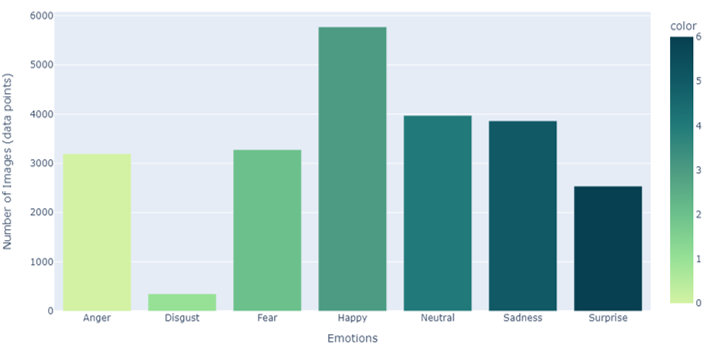
\includegraphics[width=\textwidth]{Figures/Dataset distribution.png}
        \caption{Dataset distribution of data points among 7 classes of emotions}
        \label{fig:datasetdistr}
    \end{subfigure}
    %----------------------------------------%
    \begin{subfigure}{0.22\textwidth}
        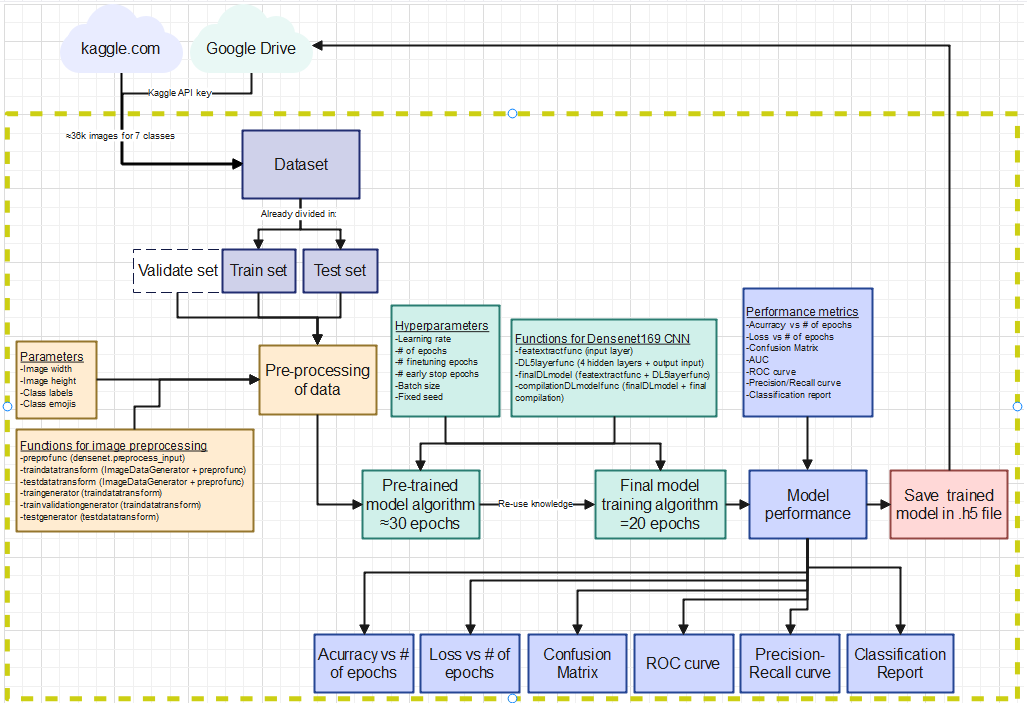
\includegraphics[width=\textwidth]{Figures/Trans_learn_workflow.png}
        \caption{Workflow for the Deep learning model with Transfer Learning)}
        \label{fig:workflow_DLTL}
    \end{subfigure}
    \begin{subfigure}{0.22\textwidth}
        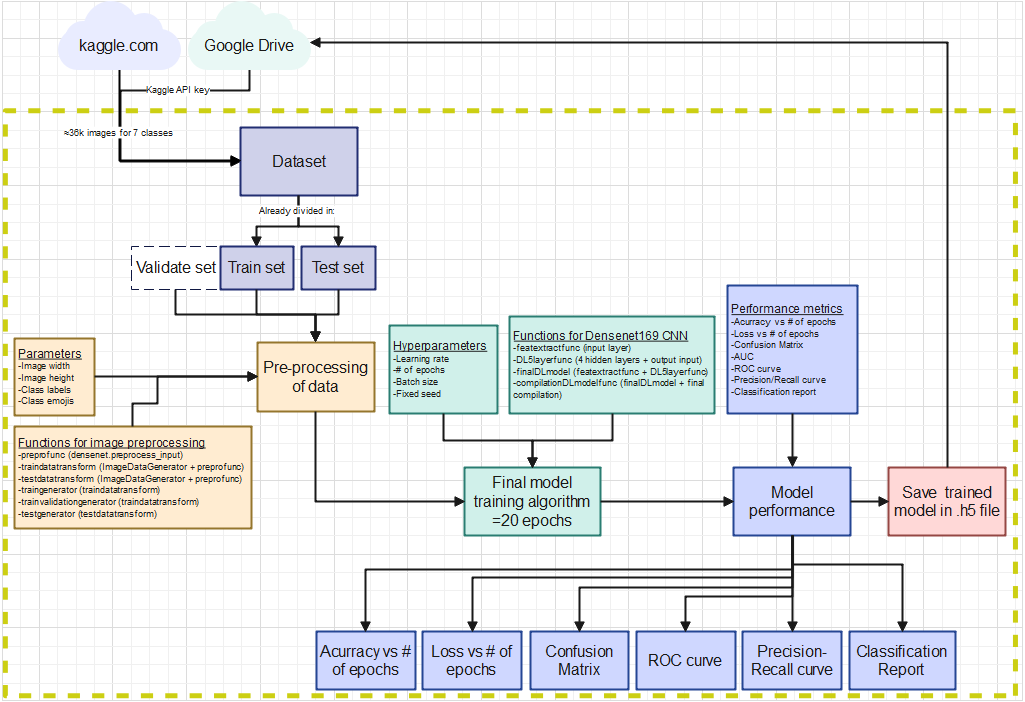
\includegraphics[width=\textwidth]{Figures/no_Trans_learn_workflow.png}
        \caption{Workflow for the Deep learning model without Transfer Learning}
        \label{fig:workflow_DLnoTL}
    \end{subfigure}
    %----------------------------------------%
    \begin{subfigure}{0.22\textwidth}
        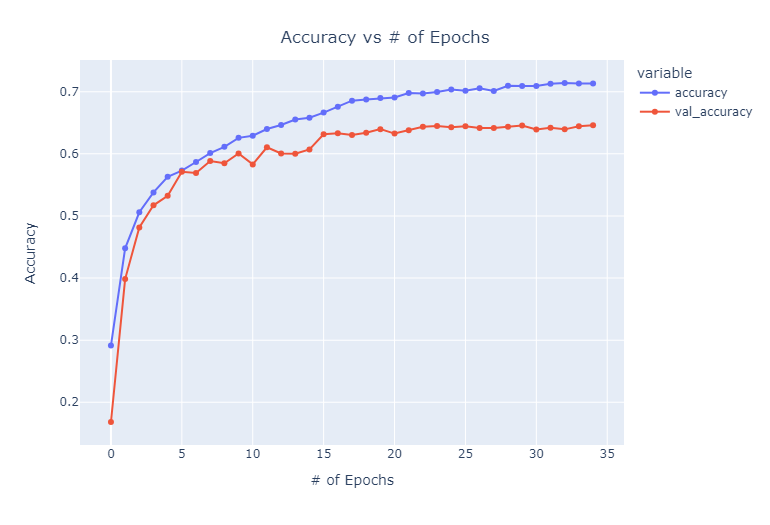
\includegraphics[width=\textwidth]{Figures/accuracyvsnumepochs.png}
        \caption{Accuracy vs. Number of Epochs (Transfer Learning)}
        \label{fig:accuracy_tl}
    \end{subfigure}
    \begin{subfigure}{0.22\textwidth}
        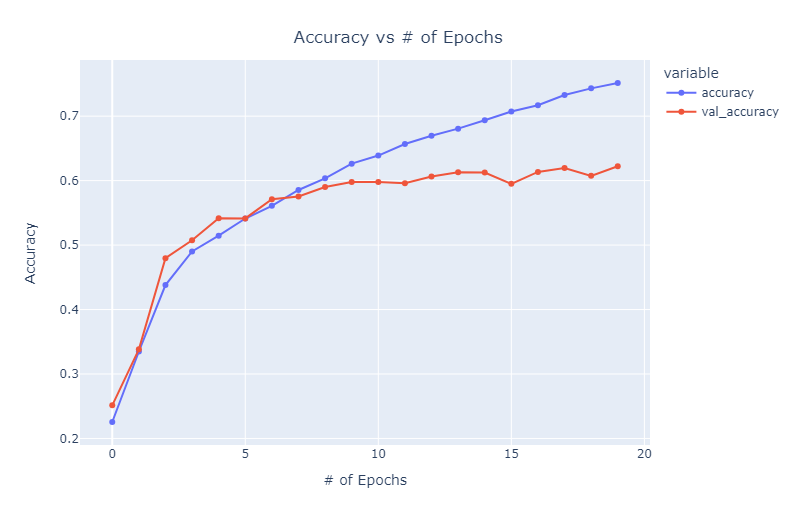
\includegraphics[width=\textwidth]{Figures/acurracy vs numepochs - no TL.png}
        \caption{Accuracy vs. Number of Epochs (No Transfer Learning)}
        \label{fig:accuracy_no_tl}
    \end{subfigure}
    %----------------------------------------%
    \begin{subfigure}{0.22\textwidth}
        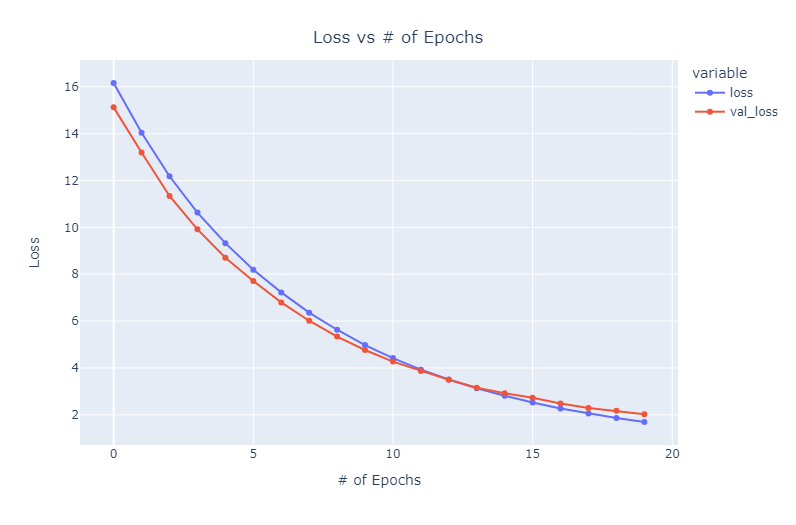
\includegraphics[width=\textwidth]{Figures/loss vs numepochs.png}
        \caption{Loss vs. Number of Epochs (Transfer Learning)}
        \label{fig:loss_tl}
    \end{subfigure}
    \begin{subfigure}{0.22\textwidth}
        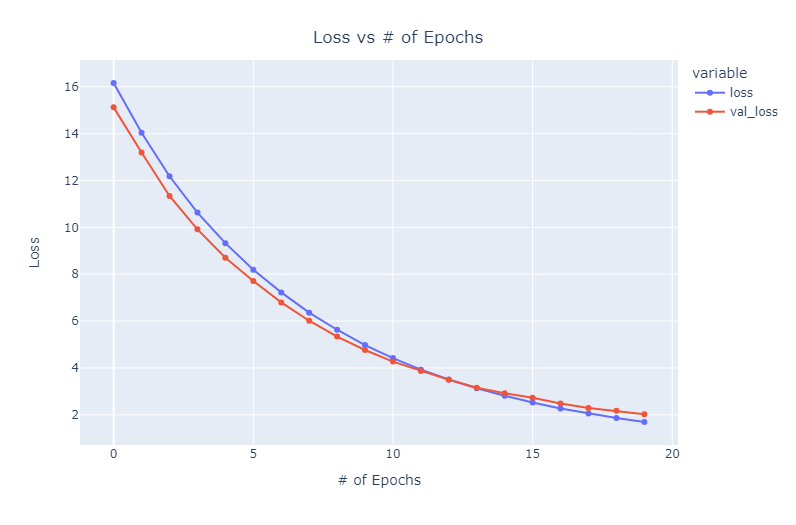
\includegraphics[width=\textwidth]{Figures/loss vs numepochs - no TL.png}
        \caption{Loss vs. Number of Epochs (No Transfer Learning)}
        \label{fig:loss_no_tl}
    \end{subfigure}
    %----------------------------------------%
    \begin{subfigure}{0.22\textwidth}
        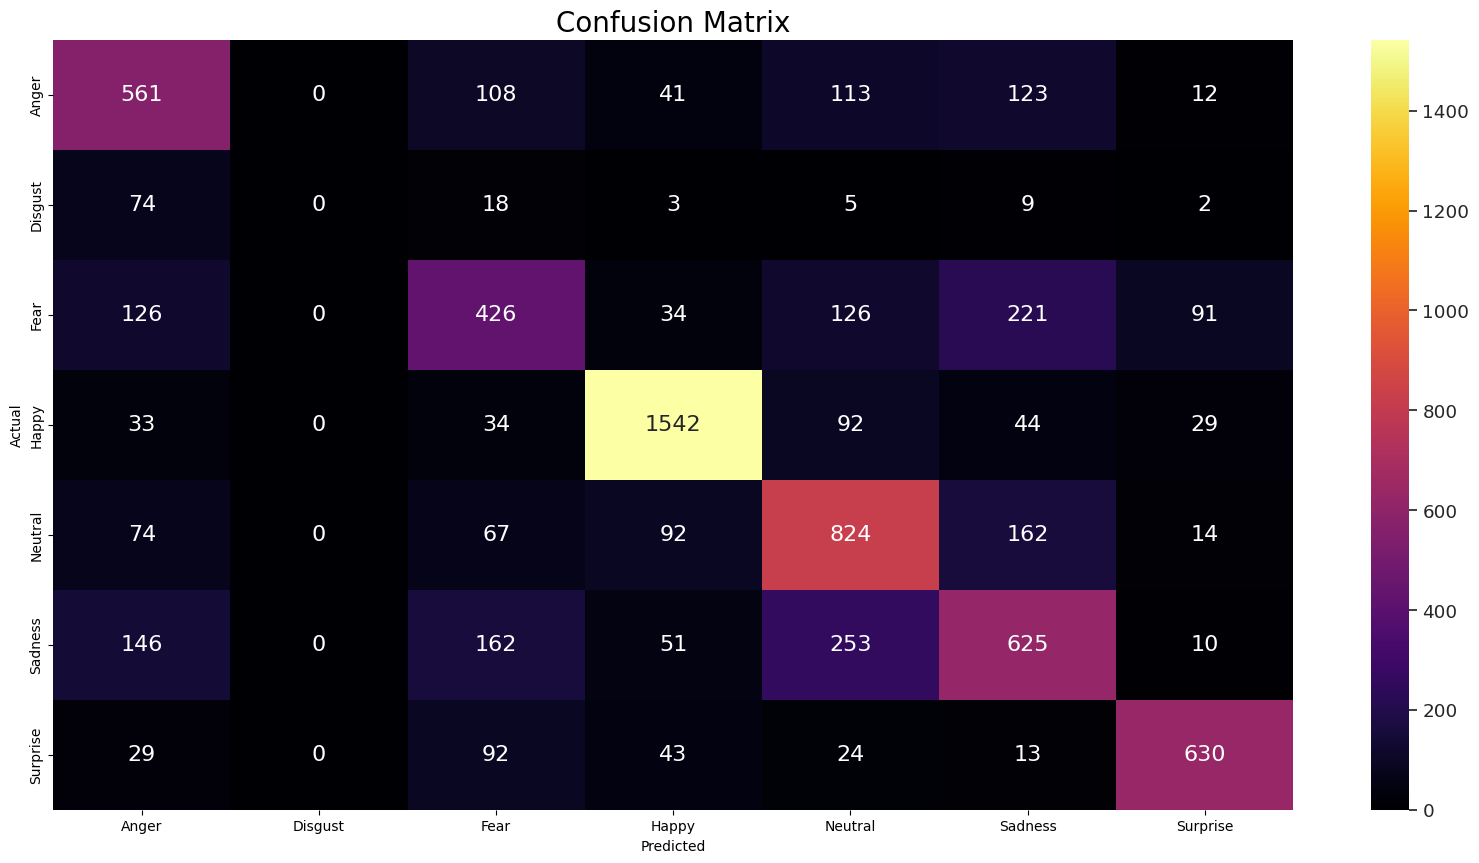
\includegraphics[width=\textwidth]{Figures/Confusion Matrix.png}
        \caption{Confusion Matrix (Transfer Learning)}
        \label{fig:confmat_tl}
    \end{subfigure}
    \begin{subfigure}{0.22\textwidth}
        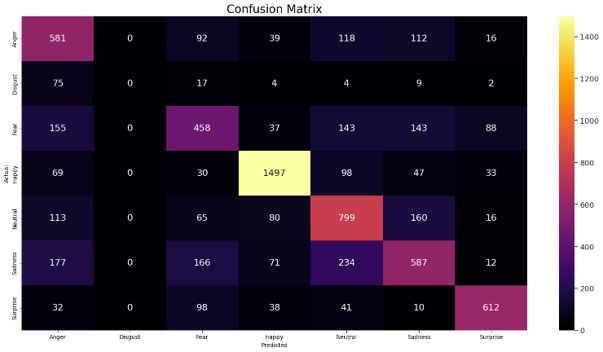
\includegraphics[width=\textwidth]{Figures/Confusion matrix - no TL.png}
        \caption{Confusion Matrix (No Transfer Learning)}
        \label{fig:confmat_no_tl}
    \end{subfigure}
    %----------------------------------------%
    \begin{subfigure}{0.22\textwidth}
        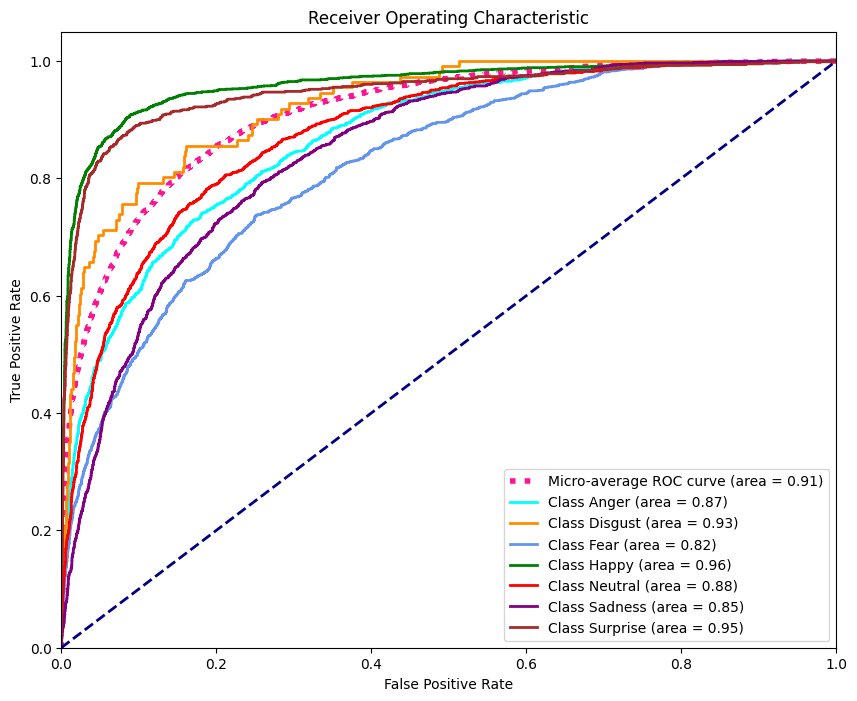
\includegraphics[width=\textwidth]{Figures/ROC.png}
        \caption{ROC (Receiver Operating Characteristic)}
        \label{fig:roc_tl}
    \end{subfigure}
    \begin{subfigure}{0.22\textwidth}
        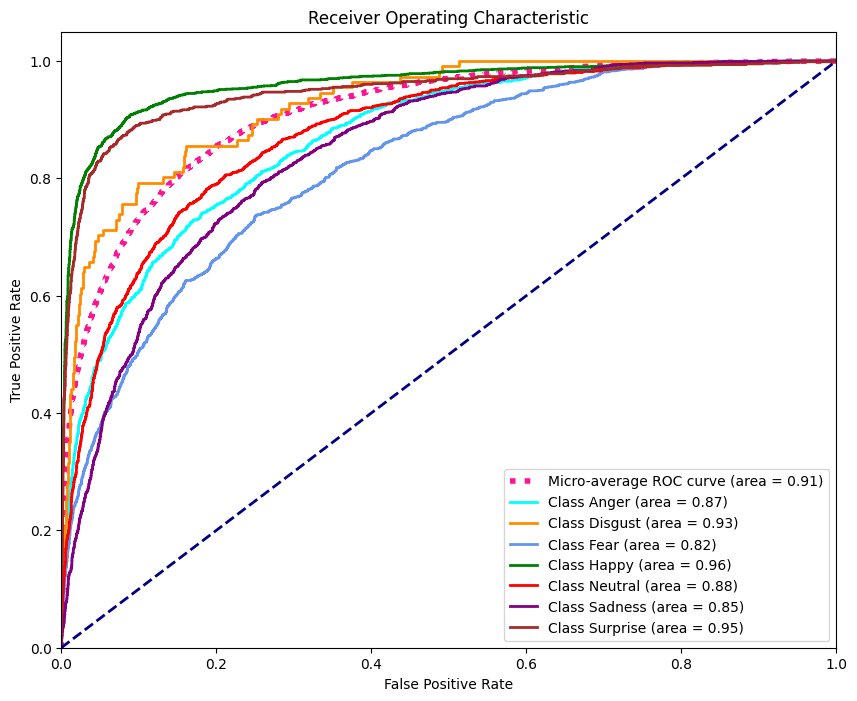
\includegraphics[width=\textwidth]{Figures/ROC - no TL.png}
        \caption{ROC (Receiver Operating Characteristic)}
        \label{fig:roc_notl}
    \end{subfigure}
    %----------------------------------------%
    \begin{subfigure}{0.22\textwidth}
        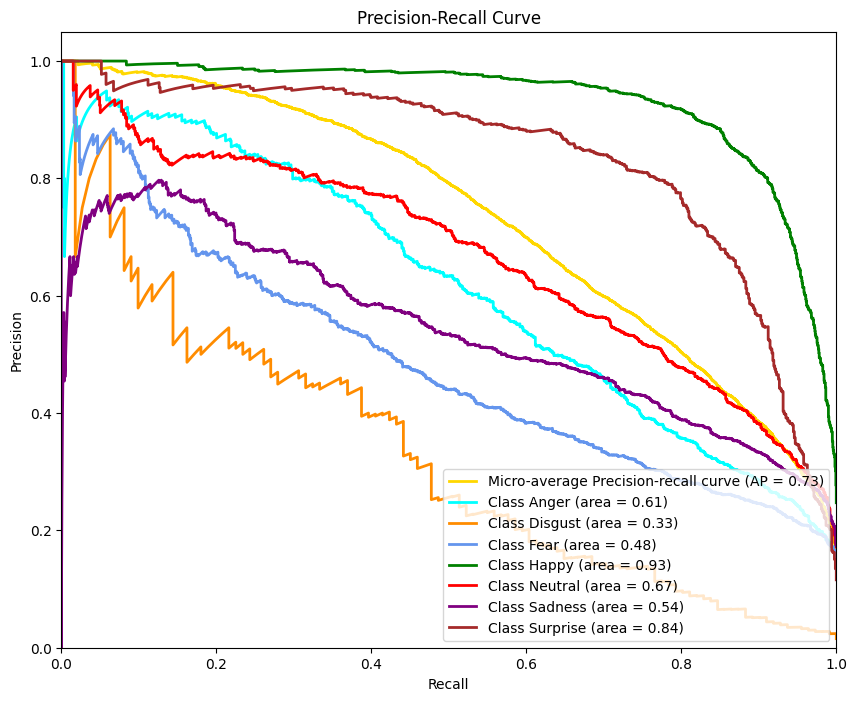
\includegraphics[width=\textwidth]{Figures/Precision-recall curve.png}
        \caption{Precision-Recall Curve (Transfer Learning)}
        \label{fig:prec_recall_tl}
    \end{subfigure}
    \begin{subfigure}{0.22\textwidth}
        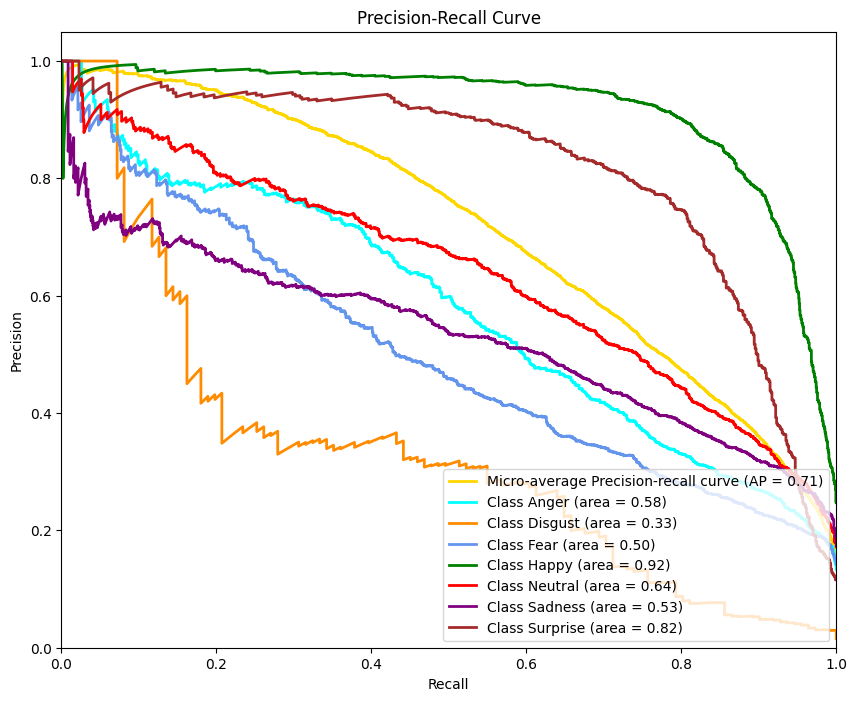
\includegraphics[width=\textwidth]{Figures/Precision-recall curve - no TL.png}
        \caption{Precision-Recall Curve (No Transfer Learning)}
        \label{fig:prec_recall_no_tl}
    \end{subfigure}
    %----------------------------------------%
    \begin{subfigure}{0.22\textwidth}
        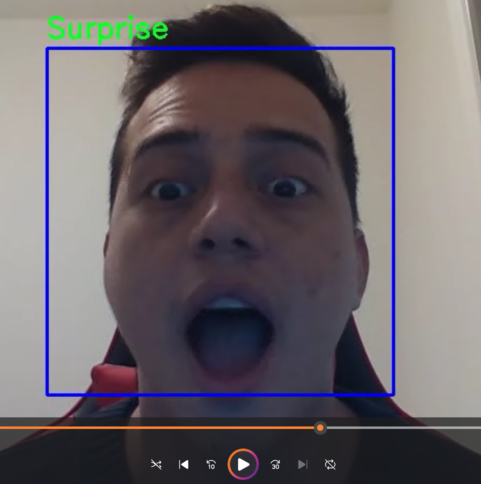
\includegraphics[width=\textwidth]{Figures/opencvsurprise.png}
        \caption{Prediction in Real-Time Analysis (Surprise)}
        \label{fig:opencvsurprise}
    \end{subfigure}
    %----------------------------------------%
    \begin{subfigure}{0.22\textwidth}
        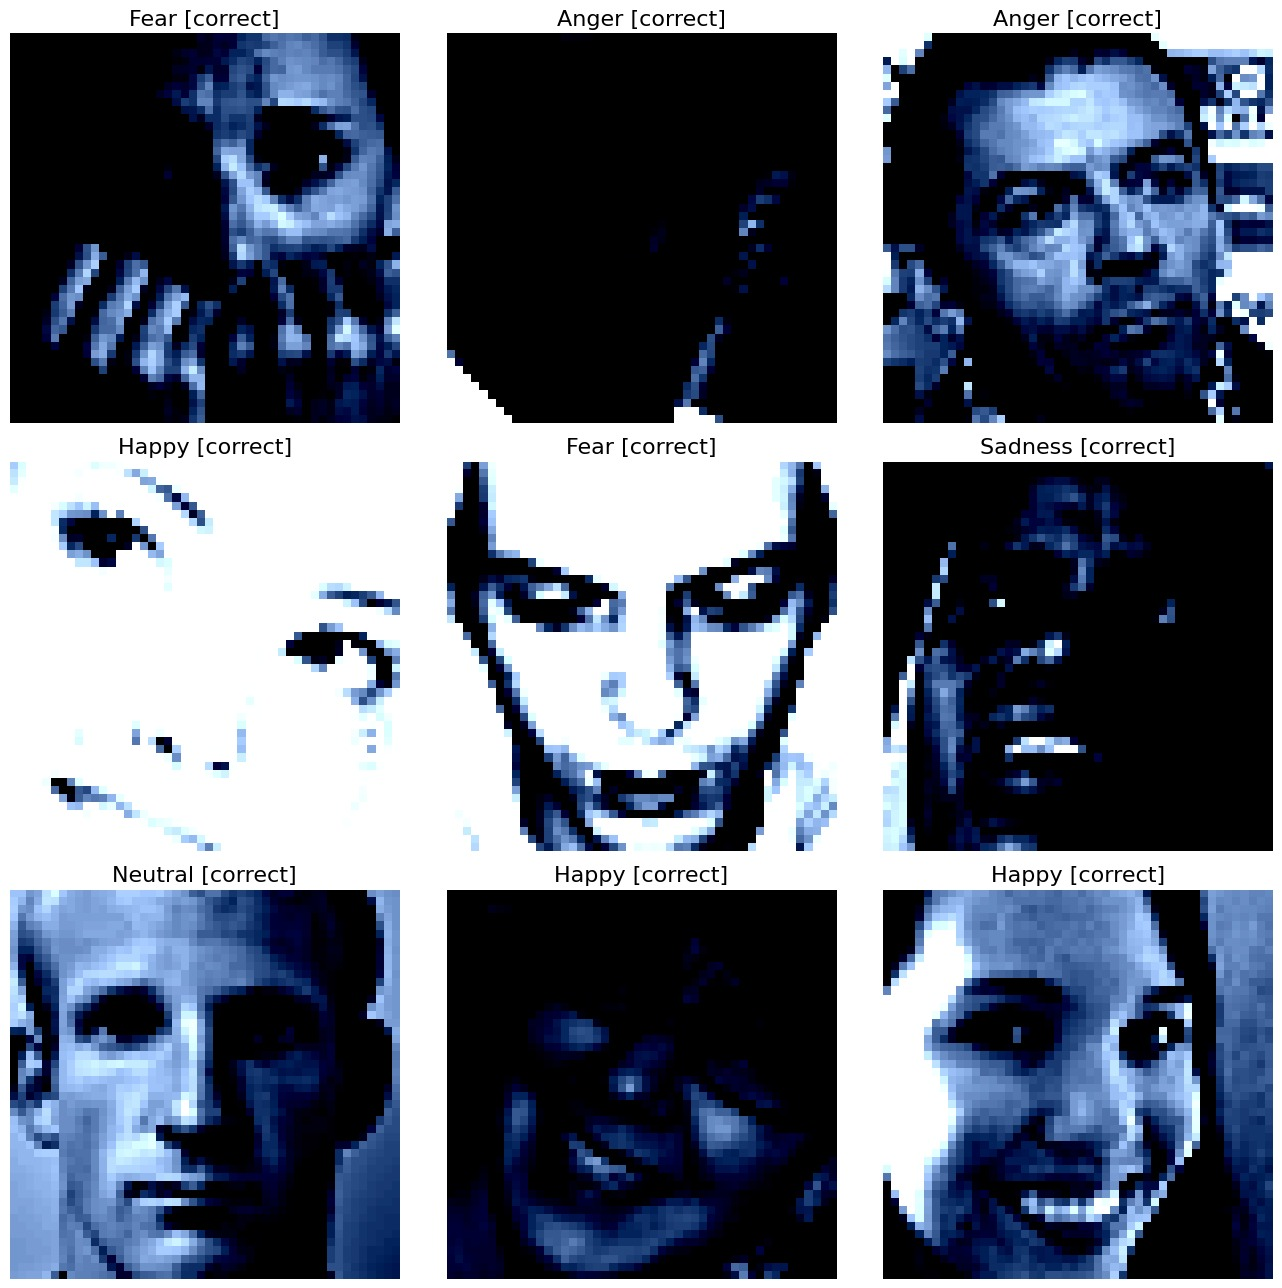
\includegraphics[width=\textwidth]{Figures/9imagepredictionTLmodel.png}
        \caption{Prediction of 9 Images with Transfer Learning}
        \label{fig:9imageprediction_TLmodel}
    \end{subfigure}
    \begin{subfigure}{0.22\textwidth}
        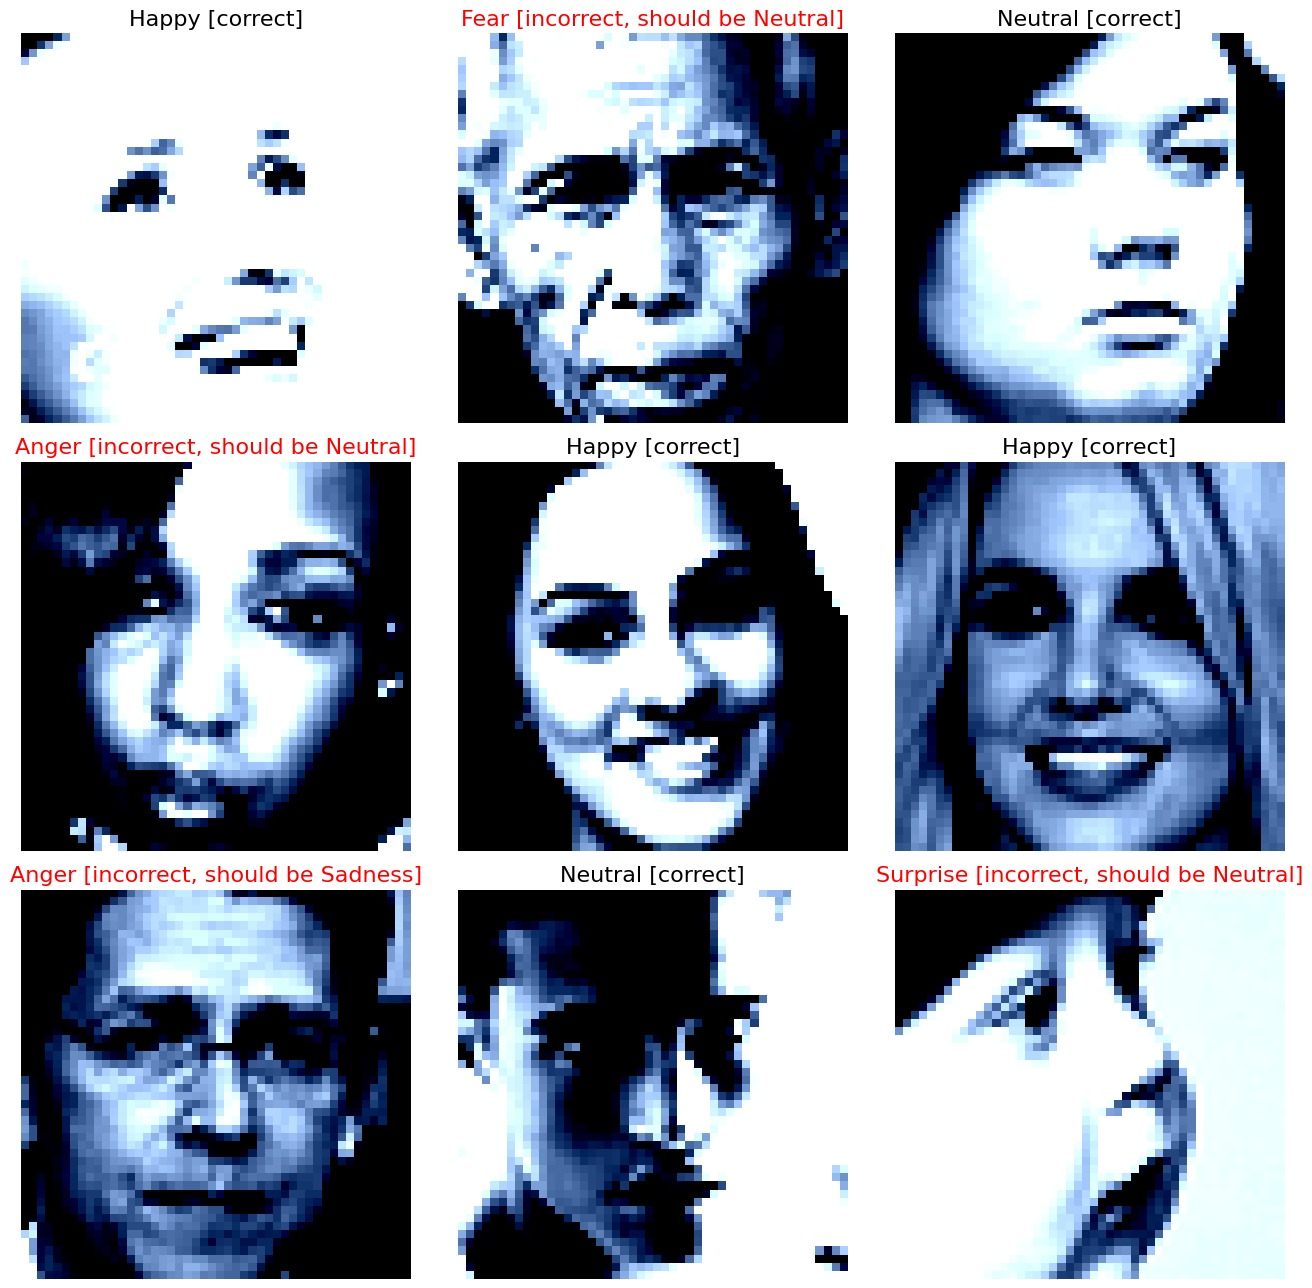
\includegraphics[width=\textwidth]{Figures/9imagepredictionNOTLmodel.png}
        \caption{Prediction of 9 Images without Transfer Learning}
        \label{fig:9imageprediction_NOTLmode}
    \end{subfigure}
    %----------------------------------------%
    \begin{subfigure}{0.22\textwidth}
        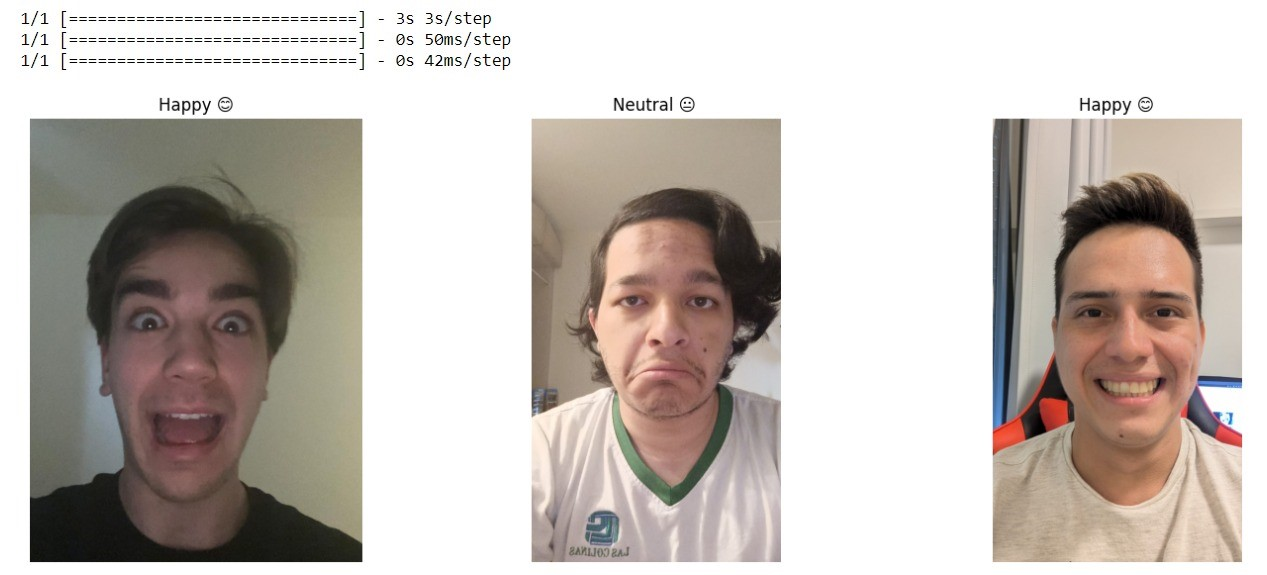
\includegraphics[width=\textwidth]{Figures/3camimageprediction.png}
        \caption{3 cam Images Prediction}
        \label{fig:3camimageprediction}
    \end{subfigure}
    \caption{Performance Comparison of DenseNet169 Model with and without Transfer Learning}
    \label{fig:results_summary}
\end{figure*}

\end{document}
